% epaData — CS396 Phase 1 project report.
% Build from the repository root: npm run report  (tectonic report/main.tex)
\documentclass[11pt,a4paper]{article}

\usepackage[margin=2.5cm]{geometry}
\usepackage{fontspec}
\usepackage{microtype}
\usepackage{amsmath,amssymb}
\usepackage{graphicx}
\usepackage{booktabs}
\usepackage{tabularx}
\usepackage{longtable}
\usepackage{array}
\usepackage{xcolor}
\usepackage{listings}
\usepackage{caption}
\usepackage{float}
\usepackage{enumitem}
\usepackage{tikz}
\usetikzlibrary{positioning,arrows.meta,shapes.multipart,fit,calc,backgrounds}
\usepackage[hidelinks]{hyperref}
\usepackage{url}
\usepackage[htt]{hyphenat}
\setlength{\emergencystretch}{2.5em}

\graphicspath{{figures/}}
\setlength{\parskip}{0.45em}
\setlength{\parindent}{0pt}
\captionsetup{font=small,labelfont=bf}
\setlist{itemsep=0.15em,topsep=0.3em}

% Chemistry and units used throughout the text.
\newcommand{\COtwo}{CO\textsubscript{2}}
\newcommand{\SOtwo}{SO\textsubscript{2}}
\newcommand{\NOx}{NO\textsubscript{x}}
\newcommand{\code}[1]{\texttt{#1}}
\newcolumntype{L}{>{\raggedright\arraybackslash}X}
\newcolumntype{R}[1]{>{\raggedright\arraybackslash}p{#1}}

% ---------------------------------------------------------------- listings
\definecolor{codebg}{RGB}{248,248,246}
\definecolor{codekw}{RGB}{0,92,158}
\definecolor{codestr}{RGB}{163,21,21}
\definecolor{codecom}{RGB}{96,120,96}
\lstset{
  basicstyle=\ttfamily\footnotesize,
  backgroundcolor=\color{codebg},
  keywordstyle=\color{codekw}\bfseries,
  stringstyle=\color{codestr},
  commentstyle=\color{codecom}\itshape,
  numbers=left, numberstyle=\tiny\color{gray}, numbersep=6pt,
  frame=single, rulecolor=\color{black!15}, framesep=4pt,
  breaklines=true, columns=fullflexible, keepspaces=true,
  showstringspaces=false, tabsize=2, captionpos=b,
  xleftmargin=1.4em, framexleftmargin=1.4em,
}
\lstdefinelanguage{TypeScript}{
  keywords={const,let,function,async,await,return,if,else,for,of,in,new,export,import,from,type,interface,true,false,undefined,null,typeof},
  sensitive=true, morecomment=[l]{//}, morecomment=[s]{/*}{*/},
  morestring=[b]", morestring=[b]', morestring=[b]`,
}
\lstdefinestyle{sql}{language=SQL, morekeywords={OVER,PARTITION,ROW_NUMBER,LIMIT,OFFSET,EXISTS,COALESCE,NULLIF,IF,REFERENCES,CASCADE,UNIQUE,INDEX}}

% ---------------------------------------------------------------- TikZ styles
\tikzset{
  box/.style={draw, rounded corners=2pt, align=center, font=\small, inner sep=5pt, fill=white},
  store/.style={box, fill=black!4},
  ext/.style={box, dashed},
  flow/.style={-{Latex[length=2mm]}, thick},
  lflow/.style={-{Latex[length=2mm]}, thick, dashed},
  lbl/.style={font=\scriptsize, fill=white, inner sep=1.5pt},
}

\title{%
  \vspace*{-1em}
  {\Large CS396 Project Phase 1 Report}\\[0.8em]
  \textbf{epaData}: A Data Management System for\\EPA Power-Sector Emissions Data}
\author{Raaj Banga \and Arnav Bawankule}
\date{October 2026}

\begin{document}
\maketitle

\begin{abstract}
\noindent
epaData is a web application that retrieves annual operating and emissions data for U.S.\
power-plant units from the EPA Clean Air Markets Program Data (CAMPD) API, imports CSV and
Excel files after validating them, stores the result in a relational SQLite database, and lets
users search, rank, compare, inspect, and download it. The committed database holds 1,619
facilities, 5,204 generating units, and 50,947 unit-year records for the reporting years
2015--2026. Every record can be traced to the retrieval or file that last wrote it. Every
import, whether from the API or a file, is first compared with the stored data and is saved
only after the user approves it. Rows that fail validation are kept in a data-quality report
rather than discarded. Searches can be built from filters, from numeric ranges, or from a
plain-English description that a rule-based parser translates into the same filters. This
report describes the problem, the functions delivered, the architecture and database design,
the technologies used, the most distinctive features, the testing performed, and the
limitations that remain for Phase~2.
\end{abstract}

\tableofcontents
\newpage

% ------------------------------------------------------------------------
\section{Project description}
\label{sec:description}

\subsection{The problem}

Fossil-fuel power plants in the United States that fall under federal programs such as the
Acid Rain Program and the Cross-State Air Pollution Rule must monitor and report how much
fuel they burn, how much electricity they generate, and how much sulfur dioxide (\SOtwo),
nitrogen oxides (\NOx), and carbon dioxide (\COtwo) leave their stacks. The U.S.\
Environmental Protection Agency publishes these reports through the Clean Air Markets Program
Data (CAMPD) service, both as downloadable files and through a REST API, the CAM API. The
data is detailed and authoritative: for every generating unit it gives annual operating time,
gross load, heat input, and emitted mass, together with the unit's fuel, type, and
pollution-control equipment.

Getting from this source to an answer is harder than it should be. A question such as
\emph{``Which coal units in Kentucky emitted more than 500{,}000 tons of \COtwo{} in 2025?''}
needs a request against the right endpoint with the right parameters, and joining the result
with facility metadata, then filtering on a numeric threshold. A comparison across years needs
one request per year. Analysts who receive CAMPD exports as spreadsheets also have no simple
way to check those files for missing values, out-of-range numbers, or repeated
facility-unit-year records before using them, or to see how a file differs from data they
already hold. And once data has been combined from several sources, it is easy to lose track
of where each number came from.

\subsection{Intended users}

The system is designed for three groups:
\begin{itemize}
  \item \textbf{Students and researchers} who need emissions data for coursework or analysis
        and want to query it without writing API code.
  \item \textbf{Environmental and energy analysts} who combine CAMPD data with their own
        spreadsheet extracts and need those files validated and reconciled with what they
        already have.
  \item \textbf{Reviewers and regulators} who must be able to trace a figure back to its
        source, see when it was retrieved, and see which records were rejected and why.
\end{itemize}
None of these users is assumed to know SQL or the structure of the CAMPD API. The interface
therefore exposes searches as forms, tables, and plain-English descriptions.

\subsection{Objectives}

The course project description defines twelve learning objectives for the full
two-phase project. Phase~1 addresses those concerned with data management:
\begin{enumerate}[label=O\arabic*.]
  \item Design a web-based information system with a front end and a database back end.
  \item Develop server routes, page templates, forms, and interactive web components.
  \item Design and implement a relational database using SQLite and an object-relational mapper.
  \item Retrieve environmental data from public sources or import downloaded files.
  \item Validate, clean, transform, and store uploaded data.
  \item Implement database search, filtering, sorting, and pagination.
  \item Export selected data and calculated results.
  \item[O11.] Test and deploy a complete data-driven web application.
  \item[O12.] Document data sources, assumptions, equations, units, and system limitations.
\end{enumerate}
Objectives O8--O10 (environmental indicators, multi-indicator scoring, and interactive charts
of evaluation results) belong to Phase~2. Section~\ref{sec:testing} returns to this list and
states, for each objective, whether it was met.

\subsection{Scope}

Phase~1 is a data-management system, not an evaluation tool. Within scope are retrieval of
annual apportioned emissions from the CAM API, upload of CSV and Excel files that follow the
CAMPD column layout, validation and storage in SQLite, search (basic, multi-constraint,
ranking, and description-based), display of facility and unit details, comparison of plants
and units, and CSV export of datasets, search results, selections, valid and invalid records,
and provenance.

Out of scope are the EPA TRACI characterisation factors~\cite{bare2011traci},
environmental-impact indicators, and
the weighted scoring model, all planned for Phase~2. Sub-annual data (hourly to monthly) is
displayed on demand from the API but not stored. The application runs locally; a hosted
deployment was considered and dropped (Section~\ref{sec:limitations}).

% ------------------------------------------------------------------------
\section{Functions implemented}
\label{sec:functions}

epaData is a single web page. Instead of separate pages, the specification's pages map to a
home view, four explorer tabs (Facilities, Units, Map, Audits), and dialogs opened from the
header: Retrieve, Upload, and Download, plus the facility, unit, and comparison dialogs opened
from the tables. Figure~\ref{fig:home} shows the home view. This section describes each
function from the user's point of view; Section~\ref{sec:design} explains how they are built.

\begin{figure}[H]
  \centering
  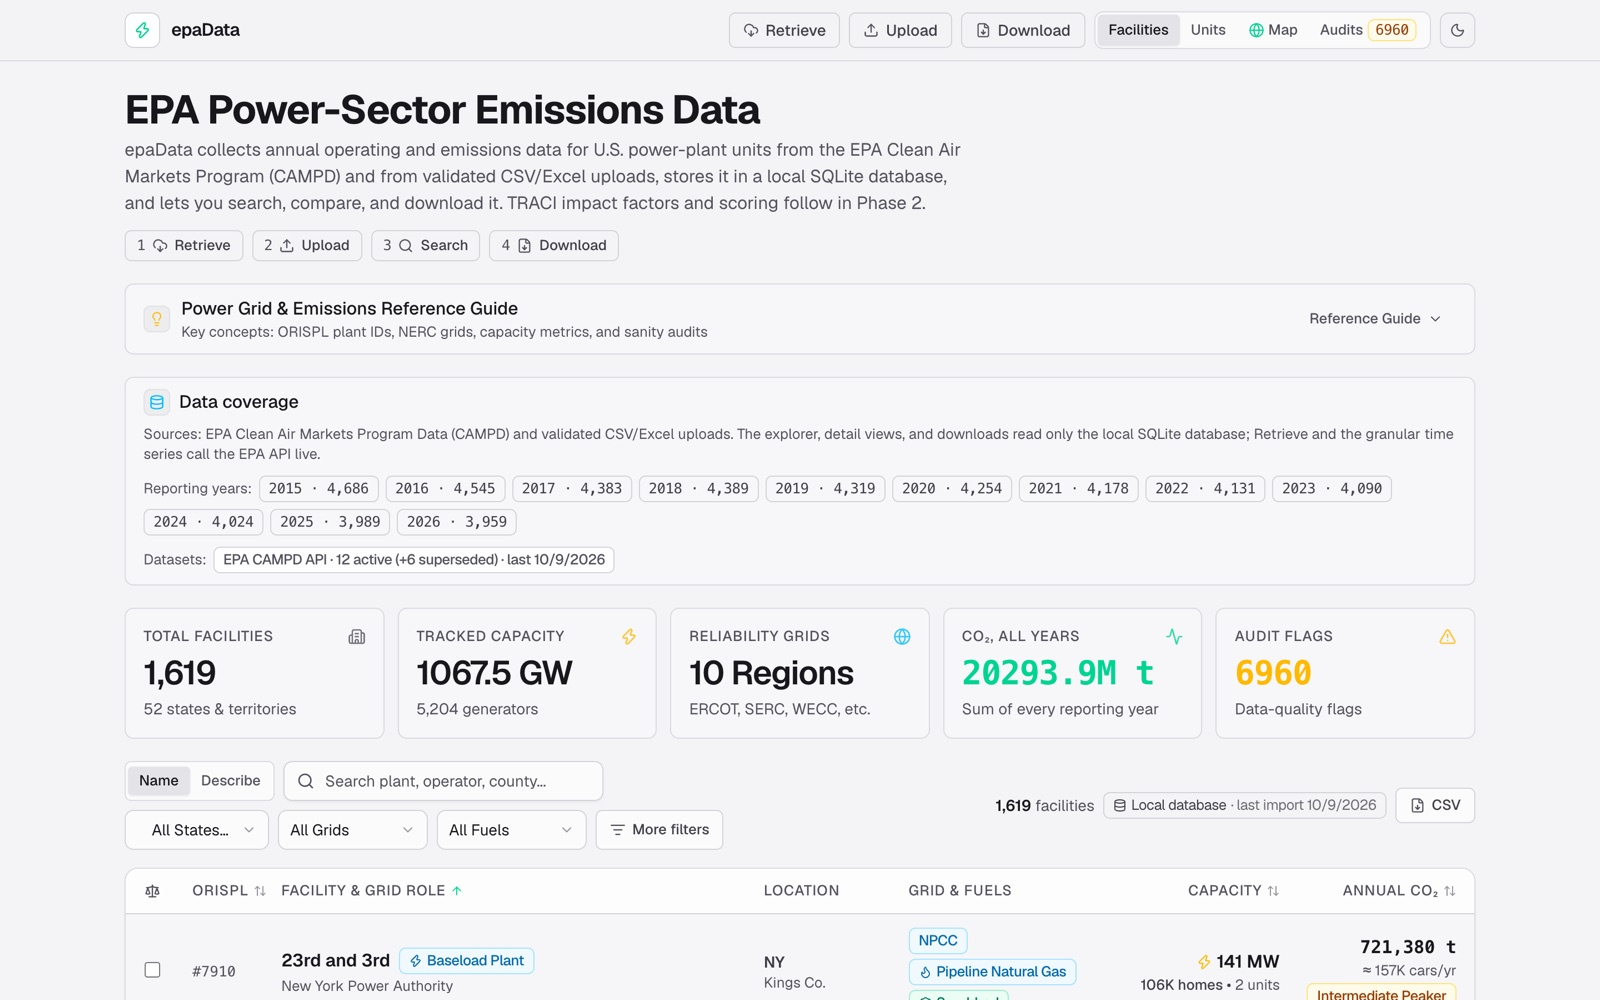
\includegraphics[width=\linewidth]{home.jpg}
  \caption{Home view: introduction, numbered links to the four main functions, data coverage
  per reporting year and source, summary tiles, and the start of the Facilities explorer.}
  \label{fig:home}
\end{figure}

\subsection{Home page}

The home view opens with a short introduction to the project and its data sources, followed
by four numbered buttons in workflow order: Retrieve, Upload, Search, and Download. A
coverage strip lists the number of unit-year records for each reporting year and summarises
the datasets by source, for example ``EPA CAMPD API $\cdot$ 12 active (+6 superseded)''. It
also states which parts of the application read the local database and which call the EPA API
live. Five tiles summarise the database: facilities, installed capacity, reliability regions,
total \COtwo{} over all years, and the number of data-quality flags.

\subsection{Data retrieval from the EPA API}

The \textbf{Retrieve} dialog names its method (EPA CAM API, apportioned annual emissions) and
offers the filters required by the specification: a range of reporting years, state, facility
IDs, fuel type, unit type, and control technology. The fuel, unit-type, and control lists are
loaded from CAMPD's master-data endpoints, so every choice is a value the API accepts. While
the user edits the form, a panel titled \emph{Already in the database} shows how many unit-years
the local database holds for those years and filters and which dataset last wrote them.

Pressing \textbf{Preview} fetches the data without saving anything. The dialog then reports,
per year, how many rows were received and how many are new, changed, unchanged, or dropped,
and lists example rows in each category. For changed rows it shows the stored and incoming
value of every field that differs. \textbf{Approve \& save} then stores the year as a new
dataset; \textbf{Cancel} discards the preview. A history table lists every past retrieval with
its parameters, date, status, and counts. The API key is read from a server-side environment
variable and never reaches the browser. Section~\ref{sec:feat-retrieve} walks through an
example.

\subsection{File upload and validation}

The \textbf{Upload} dialog accepts a CSV or Excel file up to 100\,MB, either dragged onto the
dialog or selected with a file picker. The extension and size are checked in the browser and
again on the server. A Python script then reads the file, matches its headers to the database
columns, validates every row, and detects repeated facility-unit-year records. The dialog shows
the result before anything is written:
\begin{itemize}
  \item counts of rows, valid rows, rejected rows, duplicates, and physical-sanity flags;
  \item the tables the import will write and how its records compare with the database
        (new, changed, unchanged);
  \item a row preview with a status per row, the rejected rows with the column, value, and
        reason, the duplicates and how each is resolved, and the column mapping.
\end{itemize}
The user approves or cancels. An approved import stores the valid records and the rejected
and duplicate rows. It also stores the upload's metadata and a copy of the original file.
The rejected rows can be downloaded straight from the confirmation. Section~\ref{sec:feat-upload}
shows this on the committed sample file.

\subsection{Search}

The Facilities and Units tabs share one filter bar. The Facilities tab shows one row per
plant with totals; the Units tab shows one row per unit and reporting year, the grain of the
underlying records.

\paragraph{Basic search.} A text box searches facility names, owners and operators, and
counties, and also matches a facility ID. Selects in the toolbar filter by state, NERC region,
and primary fuel; \emph{More filters} adds facility ID, unit ID, reporting year, county,
secondary fuel, unit type, \SOtwo/\NOx/PM control, operating status, audit flag and severity,
and the origin of the record (API or file upload).

\paragraph{Multi-constraint and range search.} All filters combine with AND. Under
\emph{More filters}, inclusive minimum and maximum bounds are available for reporting year,
operating time, gross load, heat input, and \COtwo, \SOtwo, and \NOx{} mass. Every active
filter is also shown as a removable chip above the table.

\paragraph{Description-based search.} A \emph{Name\,|\,Describe} switch turns the search box
into a sentence input. A description such as ``Find coal units in Kentucky with high CO2
emissions'' is translated into the same filters, which appear as chips and in the filter
controls so that the user can refine them. Words that could not be interpreted are listed
rather than ignored. Section~\ref{sec:feat-describe} describes the method.

\paragraph{Ranking and comparison.} Any metric column can be sorted. A \emph{Ranking} control
keeps the first $N$ rows of that order, overall or per state, which covers the specification's
top-$N$, bottom-$N$, and group-and-rank searches. Facilities and units can be ticked and
compared side by side (2--4 at a time). Historical searches use the year range or the unit
dialog, which lists every reporting year of a unit.

\paragraph{Result handling.} Results are paginated (10 to 100 rows per page), and every column
with a meaningful order is sortable. Each unit row opens the unit dialog. A \textbf{CSV} button
downloads every matching row, across all pages. The tab, filters, sort, and page are kept in
the URL query string, so a search can be bookmarked, shared, and reloaded.

\subsection{Facility and unit details}

Clicking a facility opens a dialog with its identification (ID, county, state, EPA and NERC
region, owner), its units with their fuels and controls, its year-by-year operation and
emissions, and its audit flags. A granular view in the same dialog shows hourly, daily,
weekly, or monthly data fetched live from the API, and yearly totals from the database. The
unit dialog (Figure~\ref{fig:unit}) shows identification, fuel and controls, programs, a table
of every reporting year with the dataset each record came from, and any sanity flags.

\subsection{Comparison, map, and audits}

The comparison dialog (Figure~\ref{fig:compare}) places two to four facilities or units side
by side for the latest reporting year: capacity, generation, operating hours, capacity factor,
carbon intensity, heat rate, fuels, and control coverage. The Map tab draws every facility
with coordinates either on a three-dimensional globe or on a two-dimensional Leaflet map,
sized by capacity or \COtwo{} and coloured by fuel (Figure~\ref{fig:map}). The Audits tab
lists every physical-sanity flag with its rule, severity, and explanation, paginated and
filterable.

\begin{figure}[H]
  \centering
  \begin{minipage}[t]{0.49\linewidth}
    \centering
    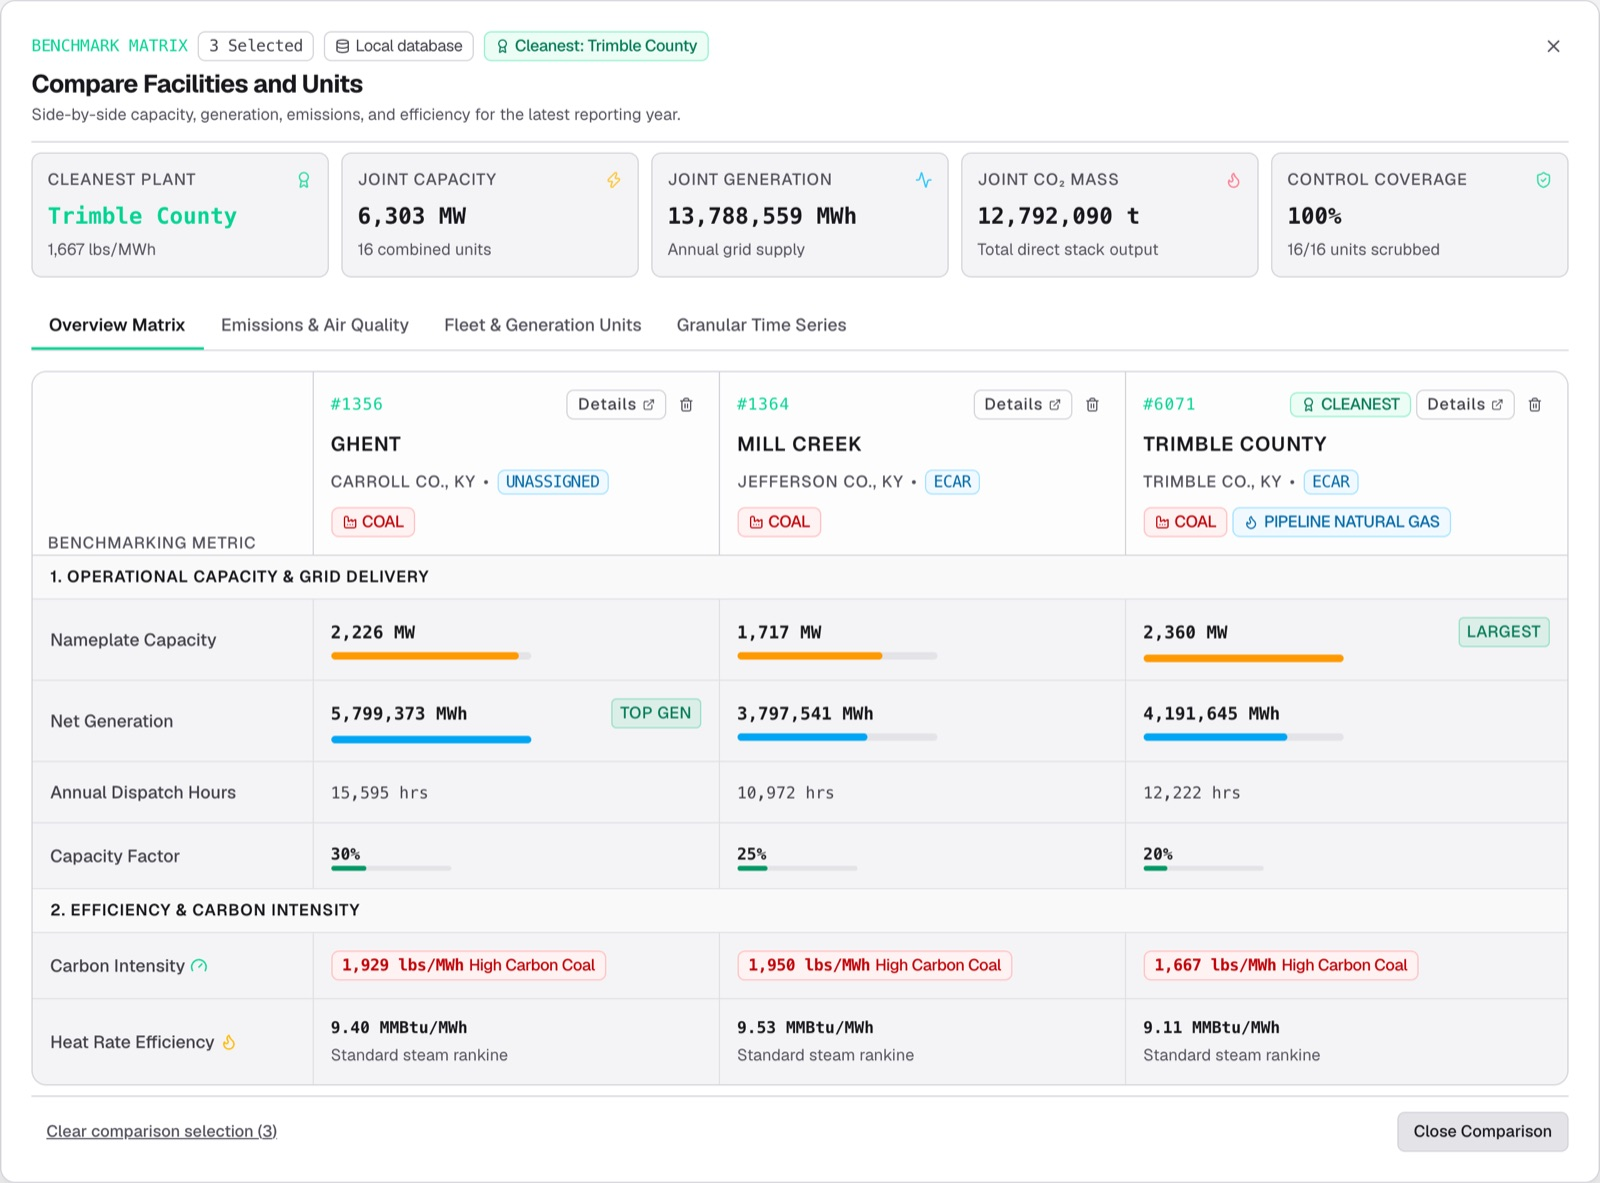
\includegraphics[width=\linewidth]{compare.jpg}
    \caption{Comparison of three Kentucky plants.}
    \label{fig:compare}
  \end{minipage}\hfill
  \begin{minipage}[t]{0.49\linewidth}
    \centering
    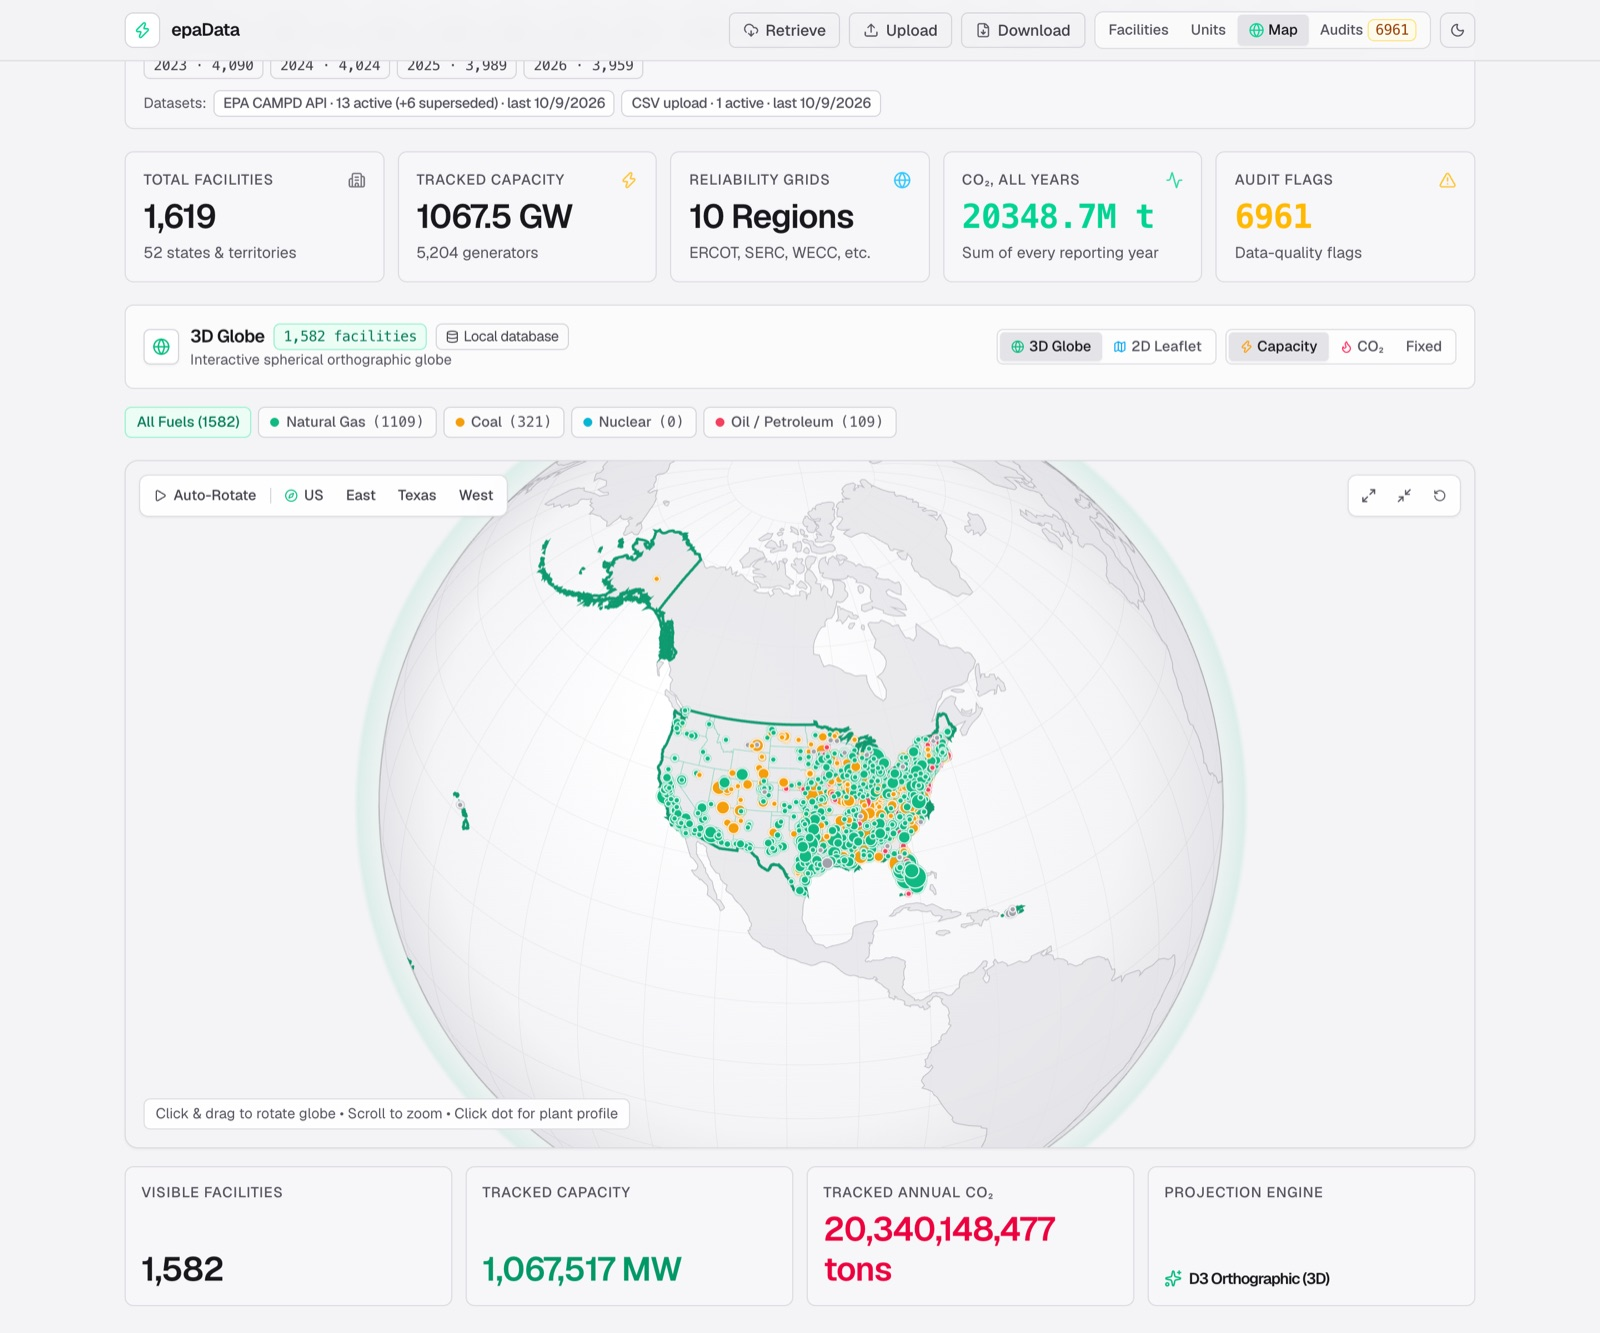
\includegraphics[width=\linewidth]{map.jpg}
    \caption{Map tab: globe view, coloured by fuel.}
    \label{fig:map}
  \end{minipage}
\end{figure}

\subsection{Download}

The \textbf{Download} dialog (Figure~\ref{fig:download}) offers the six exports the
specification requires, all as CSV: a complete dataset; its valid records; its invalid-record
report (rejected and duplicate rows with their original columns, plus records flagged by a
sanity rule); the current search results; a selection of facilities or units; and the
provenance table, one row per dataset with source, date, parameters, and counts.

\subsection{Requirement traceability}

Table~\ref{tab:trace} maps each requirement of the course project description and
each rubric item to the function that satisfies it.

{\small
\begin{longtable}{@{}R{0.3\linewidth}R{0.52\linewidth}R{0.1\linewidth}@{}}
\caption{Requirements and where epaData meets them.}\label{tab:trace}\\
\toprule
\textbf{Requirement} & \textbf{Implementation} & \textbf{Status}\\
\midrule\endfirsthead
\toprule
\textbf{Requirement} & \textbf{Implementation} & \textbf{Status}\\
\midrule\endhead
\S5 Retrieval via CAM API, key on server & Retrieve dialog; \code{CAMPD\_API} read only on the server & Met\\
\S5 Filters: year, state, facility, fuel, unit type, control & Retrieve parameters & Met\\
\S5 Preserve source, date, parameters, counts, year & \code{datasets} row per year; history table & Met\\
\S6 Steps 1--11 of the upload process & Upload dialog, \code{parse\_import.py}, approval step, archive & Met\\
\S6 Never discard invalid records silently & \code{import\_issues}; invalid-record export & Met\\
\S7 Dataset, facility, unit, annual-record tables & Six tables, keys and cascades (Section~\ref{sec:design}) & Met\footnotemark\\
\S8.1 Basic search fields & Filter bar and \emph{More filters} & Met\\
\S8.2 Multi-criteria and range search & AND-combined filters, seven min/max ranges & Met\\
\S8.3 Top-$N$, bottom-$N$, group-and-rank, comparison, history & Ranking control, compare dialog, unit dialog, year range & Met\\
\S8.4 Readable, paginated, sortable, linked, downloadable, reproducible & Tables, pagination, unit dialog, CSV, URL state & Met\\
\S8.4 Indexes on searched fields & Fourteen secondary and unique indexes & Met\\
\S9 Six pages & Home view; Retrieve, Upload, detail, and Download dialogs; explorer tabs & Met\\
\S10 Six download types, CSV & Download dialog, \code{/api/export} & Met\\
Rubric 6: description-based search & Rule-based parser, optional language-model fallback & Met\\
\bottomrule
\end{longtable}}
\footnotetext{Control and program information is stored per unit rather than per unit-year;
see Section~\ref{sec:limitations}.}

\subsection{Planned functions not completed or changed}

Our Phase~1 proposal listed several technologies and features that changed
during development. Table~\ref{tab:changes} lists them with the reason for each change.

{\small
\begin{longtable}{@{}R{0.24\linewidth}R{0.27\linewidth}R{0.43\linewidth}@{}}
\caption{Proposal versus delivered system.}\label{tab:changes}\\
\toprule
\textbf{Proposed} & \textbf{Delivered} & \textbf{Reason}\\
\midrule\endfirsthead
\toprule
\textbf{Proposed} & \textbf{Delivered} & \textbf{Reason}\\
\midrule\endhead
Prisma ORM & Drizzle ORM & Drizzle's SQL-like query builder expresses the window functions and correlated subqueries the search needs (Section~\ref{sec:discussion}).\\
Zod and Fast-CSV for upload parsing & Python script (\code{csv}, \code{openpyxl}) & The specification requires the file to be read with Python; Excel support came with it.\\
CSV upload only & CSV and Excel & Required by the specification.\\
Leaflet map with coordinate clustering & Leaflet map with scaled markers, and a D3 globe & Not completed: markers are sized and coloured instead of clustered.\\
Anomaly detection including spikes & Three physical-sanity rules & Not completed: no year-over-year spike detection.\\
Large-dataset stress tests & Timing measurements on the full database (Section~\ref{sec:testing}) & Not completed as a separate test suite.\\
Hosted deployment & Runs locally & Dropped; SQLite on serverless hosting needed workarounds (Section~\ref{sec:limitations}).\\
--- & DB-vs-API preview, provenance, origin filter, description search, granular time series, globe & Added beyond the proposal.\\
\bottomrule
\end{longtable}}

% ------------------------------------------------------------------------
\section{System design}
\label{sec:design}

\subsection{Architecture}

epaData is a single Next.js application that contains both the user interface
and the server. Figure~\ref{fig:arch} shows its components. The browser renders React
components; the first page load is rendered on the server with the data already fetched, and
later interactions call the server through typed tRPC procedures or two plain HTTP
route handlers. On the server, every database query is built with the Drizzle ORM
and executed against a single SQLite file through the libSQL client. Two kinds of work leave
the Node.js process: reading uploaded files, which is delegated to a Python script run as a
subprocess, and calls to external services, namely the EPA CAM API and, optionally, the
OpenRouter language-model service.

\begin{figure}[H]
\centering
\resizebox{\linewidth}{!}{%
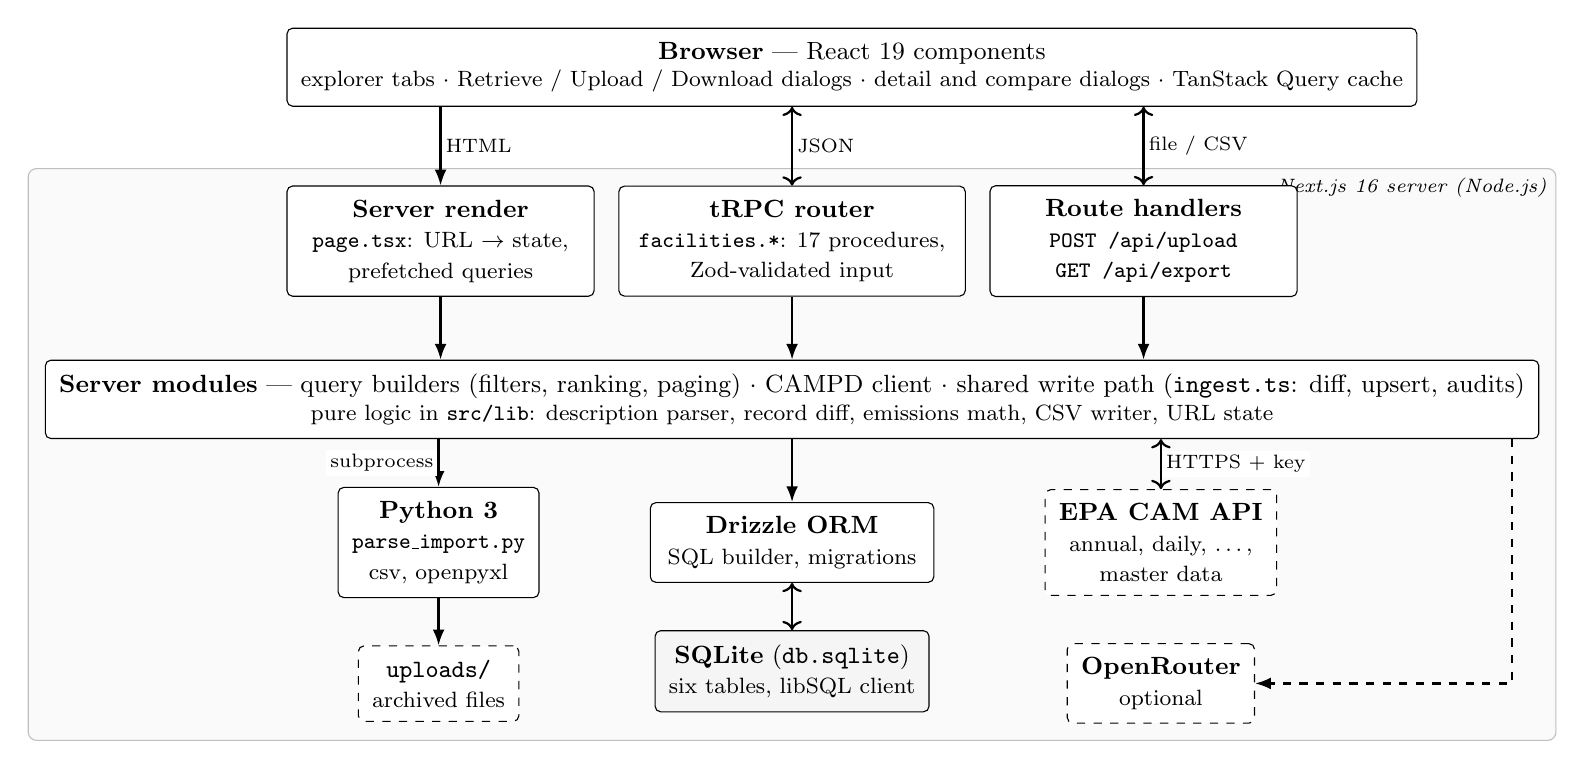
\begin{tikzpicture}[node distance=7mm and 9mm]
  % browser
  \node[box, minimum width=12.6cm] (ui) {\textbf{Browser} --- React 19 components\\[-1pt]
    {\footnotesize explorer tabs $\cdot$ Retrieve / Upload / Download dialogs $\cdot$ detail and compare dialogs $\cdot$ TanStack Query cache}};
  % server layer
  \node[box, below=10mm of ui.south west, anchor=north west, minimum width=3.9cm, minimum height=1.25cm] (rsc)
    {\textbf{Server render}\\{\footnotesize \code{page.tsx}: URL $\to$ state,}\\{\footnotesize prefetched queries}};
  \node[box, right=3mm of rsc, minimum width=4.4cm, minimum height=1.25cm] (trpc)
    {\textbf{tRPC router}\\{\footnotesize \code{facilities.*}: 17 procedures,}\\{\footnotesize Zod-validated input}};
  \node[box, right=3mm of trpc, minimum width=3.9cm, minimum height=1.25cm] (routes)
    {\textbf{Route handlers}\\{\footnotesize \code{POST /api/upload}}\\{\footnotesize \code{GET /api/export}}};
  % domain layer
  \node[box, below=8mm of trpc, minimum width=12.6cm] (lib)
    {\textbf{Server modules} --- query builders (filters, ranking, paging) $\cdot$ CAMPD client $\cdot$ shared write path (\code{ingest.ts}: diff, upsert, audits)\\[-1pt]
    {\footnotesize pure logic in \code{src/lib}: description parser, record diff, emissions math, CSV writer, URL state}};
  \node[box, below=8mm of lib, minimum width=3.6cm] (orm) {\textbf{Drizzle ORM}\\{\footnotesize SQL builder, migrations}};
  \node[store, below=6mm of orm] (db) {\textbf{SQLite} (\code{db.sqlite})\\{\footnotesize six tables, libSQL client}};
  \node[box, left=14mm of orm] (py) {\textbf{Python 3}\\{\footnotesize \code{parse\_import.py}}\\{\footnotesize csv, openpyxl}};
  \node[ext, right=14mm of orm] (epa) {\textbf{EPA CAM API}\\{\footnotesize annual, daily, \ldots,}\\{\footnotesize master data}};
  \node[ext, below=6mm of epa] (llm) {\textbf{OpenRouter}\\{\footnotesize optional}};
  \node[ext, below=6mm of py] (fs) {\code{uploads/}\\{\footnotesize archived files}};
  % background for server
  \begin{scope}[on background layer]
    \node[fit=(rsc)(trpc)(routes)(lib)(orm)(db)(py)(epa)(llm)(fs), draw=black!25, fill=black!2, rounded corners=3pt, inner sep=6pt,
      label={[font=\scriptsize\itshape, anchor=north east]north east:Next.js 16 server (Node.js)}] {};
  \end{scope}
  % arrows
  \draw[flow] (ui.south -| rsc) -- node[lbl, right]{HTML} (rsc.north);
  \draw[flow, <->] (ui.south -| trpc) -- node[lbl, right]{JSON} (trpc.north);
  \draw[flow, <->] (ui.south -| routes) -- node[lbl, right]{file / CSV} (routes.north);
  \draw[flow] (rsc.south) -- (rsc.south |- lib.north);
  \draw[flow] (trpc.south) -- (lib.north);
  \draw[flow] (routes.south) -- (routes.south |- lib.north);
  \draw[flow] (lib.south -| orm) -- (orm.north);
  \draw[flow, <->] (orm) -- (db);
  \draw[flow] (lib.south -| py) -- node[lbl, left]{subprocess} (py.north);
  \draw[flow, <->] (lib.south -| epa) -- node[lbl, right]{HTTPS + key} (epa.north);
  \draw[lflow] ($(lib.south east)+(-0.35,0)$) |- (llm.east);
  \draw[flow] (py) -- (fs);
\end{tikzpicture}}
\caption{Architecture. Solid boxes run inside the Next.js server process; dashed boxes are
external services or files. The browser never talks to the EPA API or OpenRouter directly,
so their keys stay on the server.}
\label{fig:arch}
\end{figure}

The code is organised in layers that mirror the figure. \code{src/app} contains the page and
its React components. \code{src/server/api} defines the tRPC router, whose procedures validate
their input with Zod and delegate to \code{src/server}. That directory holds the
query builders, the CAMPD client, the upload and export modules, and the shared write path.
\code{src/lib} contains logic with no database or network access: filter and URL state, the
description parser, record comparison, emissions arithmetic, and CSV formatting. Keeping this
logic pure is what makes it testable with plain unit tests (Section~\ref{sec:testing}). The
same modules are used by the command-line scripts in \code{scripts/}, so the CLI sync and the
in-app retrieval run identical code.

\subsection{Life cycle of a search}

Following one search through the system shows how the components interact. Suppose a user
opens the Units tab, chooses Kentucky and Coal, sets the year to 2025, and enters a minimum
\COtwo{} of 500{,}000~tons.

\begin{enumerate}
  \item Each change updates a filter object held in React state. A pure function,
        \code{explorerSearchParams}, mirrors the object into the URL, so the browser history
        and any shared link carry the full search:\\[2pt]
        {\small\code{?tab=units\&stateCode=KY\&primaryFuel=Coal\&year=2025\&co2MassTonsMin=500000}}
  \item A deferred copy of the filters is passed to \code{api.facilities.getUnitYears.useQuery}.
        Deferring lets typing stay responsive; TanStack Query keeps the previous page on screen
        until the new one arrives and caches each distinct query.
  \item On the server, Zod validates the input against \code{facilityFilterSchema} extended
        with paging and sort fields, rejecting unknown sort keys or out-of-range page sizes.
  \item \code{rankedUnitYears} builds one SQL statement: \code{annual\_records} joined to
        \code{units}, \code{facilities}, and \code{datasets}; a WHERE clause assembled from
        three condition builders (facility, unit, and record conditions); and a
        \code{ROW\_NUMBER()} window over the requested sort. Listing~\ref{lst:rank} in
        Section~\ref{sec:feat-ranking} shows the generated SQL.
  \item \code{pageOf} runs two queries over the same ranked subquery, one for the page of
        rows and one for the total count, and returns both. SQLite answers in about 5\,ms
        using the \code{(year, co2\_mass\_tons)} index.
  \item The table renders 25 rows across three pages. The \textbf{CSV} button links to
        \code{/api/export?type=search\&\ldots} with the same query string. That handler parses
        the string with the same \code{parseExplorerParams} function and runs the same
        \code{rankedUnitYears} without a page limit, so the file contains exactly the rows the
        table showed.
\end{enumerate}

When the page is reloaded, \code{page.tsx} parses the URL on the server, prefetches the same
query, and sends the rendered table with the data embedded, so a shared link opens directly on
the results.

\subsection{Database schema}

Figure~\ref{fig:er} shows the six tables and their relationships. Following the relational
model~\cite{codd1970}, each table holds one kind of entity, identified by a key, and
relationships are expressed through foreign keys. The design follows the real-world hierarchy
of the data: a \emph{facility} (a power plant, identified by its EPA
ORISPL code) houses one or more \emph{units} (boilers, turbines, or engines), and each unit
reports one \emph{annual record} per year. Two tables record where data came from:
\emph{datasets} has one row per retrieval or upload, and \emph{import\_issues} has one row per
source row that was rejected or skipped. A sixth table, \emph{data\_audit\_logs}, holds the
physical-sanity flags raised on annual records.

\begin{figure}[H]
\centering
\resizebox{\linewidth}{!}{%
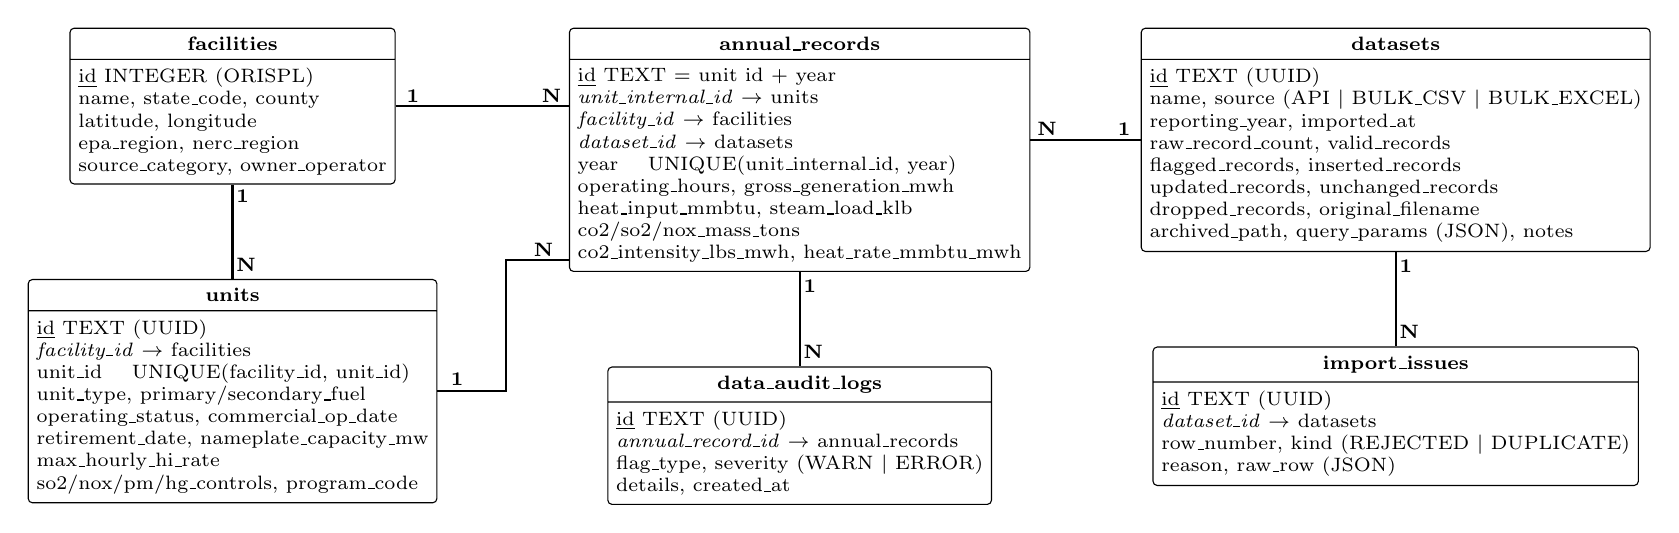
\begin{tikzpicture}[
  ent/.style={rectangle split, rectangle split parts=2, draw, rounded corners=1.5pt,
    font=\scriptsize, align=left, inner sep=3pt, fill=white,
    rectangle split part fill={black!8,white}},
  rel/.style={thick},
  card/.style={font=\scriptsize\bfseries, inner sep=1pt},
]
  \node[ent] (fac) {\textbf{facilities}
    \nodepart{second}
    \underline{id} INTEGER (ORISPL)\\
    name, state\_code, county\\
    latitude, longitude\\
    epa\_region, nerc\_region\\
    source\_category, owner\_operator};
  \node[ent, below=12mm of fac] (unit) {\textbf{units}
    \nodepart{second}
    \underline{id} TEXT (UUID)\\
    \textit{facility\_id} $\to$ facilities\\
    unit\_id \quad UNIQUE(facility\_id, unit\_id)\\
    unit\_type, primary/secondary\_fuel\\
    operating\_status, commercial\_op\_date\\
    retirement\_date, nameplate\_capacity\_mw\\
    max\_hourly\_hi\_rate\\
    so2/nox/pm/hg\_controls, program\_code};
  \node[ent, right=22mm of fac.north east, anchor=north west] (ar) {\textbf{annual\_records}
    \nodepart{second}
    \underline{id} TEXT = unit id + year\\
    \textit{unit\_internal\_id} $\to$ units\\
    \textit{facility\_id} $\to$ facilities\\
    \textit{dataset\_id} $\to$ datasets\\
    year \quad UNIQUE(unit\_internal\_id, year)\\
    operating\_hours, gross\_generation\_mwh\\
    heat\_input\_mmbtu, steam\_load\_klb\\
    co2/so2/nox\_mass\_tons\\
    co2\_intensity\_lbs\_mwh, heat\_rate\_mmbtu\_mwh};
  \node[ent, right=14mm of ar.north east, anchor=north west] (ds) {\textbf{datasets}
    \nodepart{second}
    \underline{id} TEXT (UUID)\\
    name, source (API $|$ BULK\_CSV $|$ BULK\_EXCEL)\\
    reporting\_year, imported\_at\\
    raw\_record\_count, valid\_records\\
    flagged\_records, inserted\_records\\
    updated\_records, unchanged\_records\\
    dropped\_records, original\_filename\\
    archived\_path, query\_params (JSON), notes};
  \node[ent, below=12mm of ar] (log) {\textbf{data\_audit\_logs}
    \nodepart{second}
    \underline{id} TEXT (UUID)\\
    \textit{annual\_record\_id} $\to$ annual\_records\\
    flag\_type, severity (WARN $|$ ERROR)\\
    details, created\_at};
  \node[ent, below=12mm of ds] (iss) {\textbf{import\_issues}
    \nodepart{second}
    \underline{id} TEXT (UUID)\\
    \textit{dataset\_id} $\to$ datasets\\
    row\_number, kind (REJECTED $|$ DUPLICATE)\\
    reason, raw\_row (JSON)};

  \draw[rel] (fac.south) -- node[card, right, pos=0.12]{1} node[card, right, pos=0.85]{N} (unit.north);
  \draw[rel] (fac.east) -- node[card, above, pos=0.1]{1} node[card, above, pos=0.9]{N} (fac.east -| ar.west);
  \draw[rel] (unit.east) -| ($(ar.west)+(-8mm,-14mm)$) -- node[card, above, pos=0.6]{N} ($(ar.west)+(0,-14mm)$);
  \node[card] at ($(unit.east)+(2.5mm,1.5mm)$) {1};
  \draw[rel] (ar.east |- ds.west) -- node[card, above, pos=0.15]{N} node[card, above, pos=0.85]{1} (ds.west);
  \draw[rel] (ar.south) -- node[card, right, pos=0.15]{1} node[card, right, pos=0.85]{N} (log.north);
  \draw[rel] (ds.south) -- node[card, right, pos=0.15]{1} node[card, right, pos=0.85]{N} (iss.north);
\end{tikzpicture}}
\caption{Entity-relationship diagram. Underlined columns are primary keys; italic columns are
foreign keys (arrows name the referenced table). All foreign keys cascade on delete.}
\label{fig:er}
\end{figure}

\paragraph{Keys and integrity rules.} Each table enforces the rules of its domain in the
database rather than only in application code:
\begin{itemize}
  \item \code{facilities.id} is the EPA facility ID itself. The identifier is stable and
        meaningful, so it serves directly as the primary key, and URLs and exports can use it.
  \item A unit is identified within its facility by EPA's unit ID (``1'', ``CT1'', \ldots),
        which is not unique across facilities. The table therefore has a surrogate UUID key
        and a unique index on \code{(facility\_id, unit\_id)}; upserts use that pair as their
        conflict target.
  \item An annual record is unique per \code{(unit\_internal\_id, year)}, the
        ``facility-unit-year'' of the specification. Its primary key is derived from the same
        pair (\code{\$\{unitInternalId\}\_\$\{year\}}), so re-importing a year updates the
        existing row instead of inserting a duplicate.
  \item Metric columns are \code{REAL NOT NULL DEFAULT 0}. Missing CAMPD values become 0,
        so sums and ranges never meet \code{NULL}. The two derived rates are nullable,
        because they are undefined when gross load is zero.
  \item Foreign keys cascade on delete: deleting a facility removes its units and records,
        and deleting a dataset removes its issues and the records it last wrote.
\end{itemize}

\paragraph{Indexes.} Table~\ref{tab:indexes} lists the indexes and the searches they serve.
One of them, \code{(facility\_id, year)}, was added after profiling; Section~\ref{sec:testing}
explains why.

\begin{table}[H]
\centering\small
\caption{Secondary and unique indexes.}
\label{tab:indexes}
\begin{tabularx}{\linewidth}{@{}lL@{}}
\toprule
\textbf{Index} & \textbf{Serves}\\
\midrule
\code{facilities(state\_code)}, \code{(name)}, \code{(county)}, \code{(nerc\_region)}, \code{(source\_category)} & Basic-search filters and name sorting\\
\code{units(facility\_id, unit\_id)} UNIQUE & Unit identity; upsert target\\
\code{units(facility\_id)}, \code{(primary\_fuel)}, \code{(operating\_status)} & Joins and unit filters\\
\code{annual\_records(unit\_internal\_id, year)} UNIQUE & Facility-unit-year identity; upsert target; unit history\\
\code{annual\_records(year, co2\_mass\_tons)} & Year filter and \COtwo{} ranking\\
\code{annual\_records(facility\_id, year)} & Per-facility totals, overall or within one year\\
\code{data\_audit\_logs(annual\_record\_id)}, \code{import\_issues(dataset\_id)} & Flags per record; issues per dataset\\
\bottomrule
\end{tabularx}
\end{table}

\paragraph{Normalisation and one deliberate deviation.} The schema is in third normal form
with one exception: \code{annual\_records.facility\_id} repeats information derivable through
\code{units}. The redundancy lets per-facility aggregates read a single indexed table instead
of joining through units for each of the 1,619 facilities. The specification places
\SOtwo, \NOx, and PM control information and the program code on the annual record; epaData
stores them on the unit, because CAMPD reports them per unit and they rarely change from year
to year. Section~\ref{sec:limitations} discusses the consequence.

\subsection{Data flow and provenance}

Figure~\ref{fig:dataflow} shows how data enters and leaves the database. There are three ways
in, all converging on one write path in \code{src/server/ingest.ts}: the Retrieve dialog, the
Upload dialog, and the \code{sync:campd} command-line script. Before writing, the write path
loads the stored metrics of every incoming facility-unit-year and classifies each record as
new, changed, or unchanged. It then upserts facilities, units, and annual records, computes
the two derived rates, and replaces the record's sanity flags. Finally it records the counts on
the dataset row. Source rows that fail validation or repeat a facility-unit-year are written to
\code{import\_issues} with their original values and a reason.

\begin{figure}[H]
\centering
\resizebox{\linewidth}{!}{%
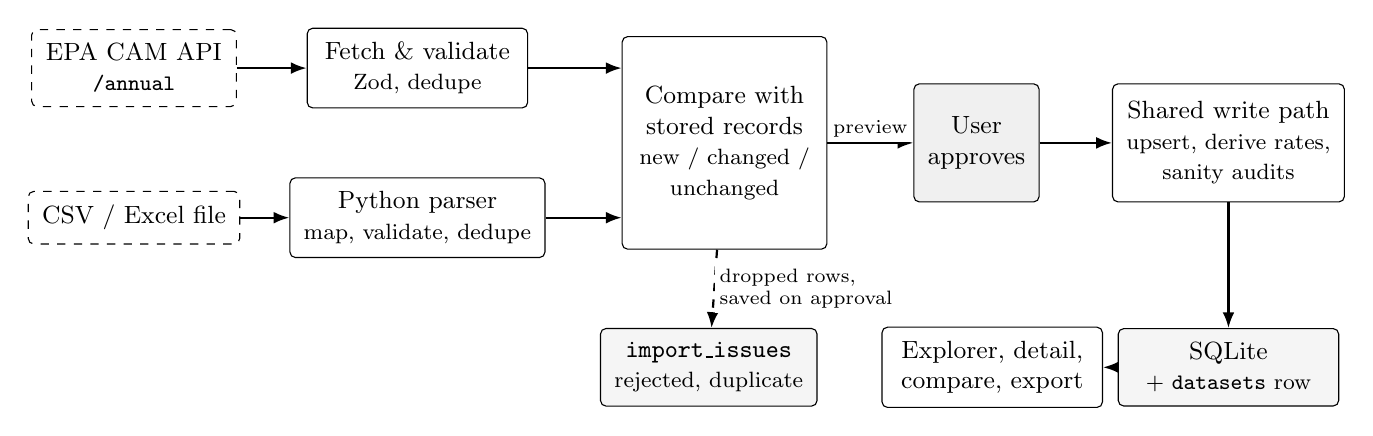
\begin{tikzpicture}[font=\small]
  \node[ext, minimum width=2.6cm] (api) at (0,0) {EPA CAM API\\{\footnotesize \code{/annual}}};
  \node[ext, minimum width=2.6cm] (file) at (0,-1.9) {CSV / Excel file};
  \node[box, minimum width=2.8cm] (prev) at (3.6,0) {Fetch \& validate\\{\footnotesize Zod, dedupe}};
  \node[box, minimum width=2.8cm] (parse) at (3.6,-1.9) {Python parser\\{\footnotesize map, validate, dedupe}};
  \node[box, minimum width=2.6cm, minimum height=2.7cm] (diff) at (7.5,-0.95) {Compare with\\stored records\\{\footnotesize new / changed /}\\{\footnotesize unchanged}};
  \node[box, fill=black!6, minimum height=1.5cm] (ok) at (10.7,-0.95) {User\\approves};
  \node[box, minimum width=2.8cm, minimum height=1.5cm] (write) at (13.9,-0.95) {Shared write path\\{\footnotesize upsert, derive rates,}\\{\footnotesize sanity audits}};
  \node[store, minimum width=2.8cm] (db) at (13.9,-3.8) {SQLite\\{\footnotesize + \code{datasets} row}};
  \node[box, minimum width=2.8cm] (exp) at (10.9,-3.8) {Explorer, detail,\\compare, export};
  \node[store, minimum width=2.6cm] (iss) at (7.3,-3.8) {\code{import\_issues}\\{\footnotesize rejected, duplicate}};
  \draw[flow] (api) -- (prev);
  \draw[flow] (file) -- (parse);
  \draw[flow] (prev.east) -- (diff.west |- prev.east);
  \draw[flow] (parse.east) -- (diff.west |- parse.east);
  \draw[flow] (diff) -- node[lbl, above]{preview} (ok);
  \draw[flow] (ok) -- (write);
  \draw[flow] (write) -- (db);
  \draw[flow] (db) -- (exp);
  \draw[lflow] (diff) -- node[lbl, right, align=left]{dropped rows,\\saved on approval} (iss);
\end{tikzpicture}}
\caption{Data flow. Retrieval and upload differ only in how rows are obtained and validated;
comparison, approval, writing, and issue logging are shared. Nothing is written before
approval. The \code{sync:campd} script skips the approval step.}
\label{fig:dataflow}
\end{figure}

The provenance model has three levels of detail. At the record level it is a coarse form of
what Buneman et al.\ call \emph{where-provenance}~\cite{buneman2001provenance}: for each
stored record, it identifies the source from which the record was copied. Each \emph{dataset} records its source, time,
parameters (for API retrievals, the exact query as JSON), file name and archived copy (for
uploads), and the counts of rows received, stored, flagged, new, updated, unchanged, and
dropped. Each \emph{annual record} points to the dataset that last wrote it, which the
interface shows as the record's origin. Each \emph{issue} keeps a rejected or duplicate source
row verbatim. When a later retrieval takes over all records of an earlier one, the earlier
dataset is kept and labelled \emph{superseded}, so the retrieval history is never rewritten.

% ------------------------------------------------------------------------
\section{Technical details}
\label{sec:technical}

\subsection{Languages}

Three languages are used, each where it fits best. \textbf{TypeScript} is used for the user
interface, the server, the query builders, and the command-line scripts. A single typed
language across browser and server lets the tRPC router's input and output types flow into
the React components without hand-written API definitions. The compiler then rejects a call
that passes a misspelled filter or reads a field the server does not return. \textbf{SQL} is
the language of the database; most of it is generated by Drizzle, but window functions,
correlated subqueries, and the provenance conditions are written as SQL fragments embedded in
TypeScript. \textbf{Python} reads uploaded files, as the specification requires, using the
standard \code{csv} module and \code{openpyxl} for Excel workbooks.

\subsection{Database system}

The database is \textbf{SQLite}~\cite{gaffney2022sqlite}, accessed through the libSQL client
(\code{@libsql/client}). SQLite stores the whole database in one file, \code{db.sqlite}, which
is committed to the repository so that the application runs immediately after installation.
SQLite supports everything the design needs: foreign keys with cascading deletes, unique and
composite indexes, upserts (\code{INSERT \ldots{} ON CONFLICT DO UPDATE}), and window functions
such as \code{ROW\_NUMBER() OVER (PARTITION BY \ldots)}, which implement ranking. Window functions
let the database rank rows within groups in a single pass over sorted input~\cite{leis2015window},
instead of self-joins or ranking in application code. The libSQL client would also allow the same code to connect to a hosted libSQL
server by changing \code{DATABASE\_URL}, although the delivered system uses only the local file.

\subsection{Frameworks and libraries}

Table~\ref{tab:stack} lists the frameworks and libraries and the role each plays.

\begin{table}[H]
\centering\small
\caption{Frameworks and libraries.}
\label{tab:stack}
\begin{tabularx}{\linewidth}{@{}>{\raggedright\arraybackslash}p{0.27\linewidth}L@{}}
\toprule
\textbf{Component} & \textbf{Role in epaData}\\
\midrule
Next.js 16 (App Router) & Application framework: server rendering of the page, route handlers for upload and export, bundling, and the development and production servers.\\
React 19 & User-interface components: tables, filter bar, dialogs.\\
tRPC 11 & Typed remote procedure calls between browser and server; the 17 \code{facilities.*} procedures.\\
TanStack Query 5 & Client-side caching, background refetching, and loading states for tRPC calls.\\
Drizzle ORM and drizzle-kit & Schema definition in TypeScript, type-checked query building, and generated SQL migrations (six so far, in \code{drizzle/}).\\
Zod & Validation of every procedure input, of CAMPD API rows, of environment variables, and of the optional language model's output.\\
Python 3, \code{csv}, \code{openpyxl} & Reading, mapping, and validating uploaded CSV and Excel files.\\
Tailwind CSS 4 & Styling with design tokens for light and dark themes.\\
Leaflet & Two-dimensional map with CARTO/OpenStreetMap tiles.\\
D3~\cite{bostock2011d3} and TopoJSON & Orthographic globe drawn on a canvas from bundled U.S.\ and world outlines.\\
lucide-react, next-themes & Icons; theme switching.\\
\code{node:test} with tsx & Unit-test runner for TypeScript without a separate test framework.\\
ESLint, Prettier, TypeScript compiler & Static checks run by \code{npm run validate}.\\
Tectonic & Builds this report from LaTeX.\\
\bottomrule
\end{tabularx}
\end{table}

\subsection{External services}

The \textbf{EPA CAM API} provides apportioned emissions at annual, monthly,
daily, and hourly resolution, plus master-data endpoints listing valid fuel types, unit types,
and control technologies. Requests carry the API key in an \code{x-api-key} header, are made
only from the server, and are paged at 500 rows per request. A safety cap of 100 pages raises
an error instead of silently truncating a result. \textbf{OpenRouter} is an
optional gateway to hosted language models, used only as a fallback by the description search
(Section~\ref{sec:feat-describe}); without a key, the feature works with the rule-based parser
alone.

\subsection{Scripts}

The npm scripts in \code{package.json} are the entry points for setup, data maintenance, and
quality checks (Table~\ref{tab:scripts}). The three data scripts in \code{scripts/} import the
same server modules as the web application, so a command-line sync and an in-app retrieval run
the same code.

\begin{table}[H]
\centering\small
\caption{Scripts.}
\label{tab:scripts}
\begin{tabularx}{\linewidth}{@{}>{\raggedright\arraybackslash}p{0.3\linewidth}L@{}}
\toprule
\textbf{Command} & \textbf{Purpose}\\
\midrule
\code{npm run dev} / \code{build} / \code{start} & Development server; production build and server.\\
\code{npm run db:migrate} & Applies the SQL migrations in \code{drizzle/} to the database named by \code{DATABASE\_URL}.\\
\code{npm run db:generate} & Generates a migration after a change to \code{src/server/db/schema.ts}.\\
\code{npm run db:seed} & Loads facilities and units from CAMPD facility CSV files.\\
\code{npm run sync:campd} & Retrieves annual emissions for one year or a range and stores them (\code{--year}, \code{--from}, \code{--to}).\\
\code{npm test} & Runs the 39 unit tests in \code{src/lib/*.test.ts}.\\
\code{npm run validate} & Format check, lint, type check, tests, and production build.\\
\code{npm run report} & Builds this report (\code{report/main.pdf}).\\
\code{scripts/parse\_import.py FILE} & Prints the validation report of a CSV or Excel file as JSON; called by the upload endpoint.\\
\bottomrule
\end{tabularx}
\end{table}

\subsection{Configuration}

Configuration is read from environment variables defined in \code{.env}, validated at start-up
by \code{src/env.js}, and documented in \code{.env.example}. Only \code{DATABASE\_URL} is
required. \code{CAMPD\_API} enables retrieval and the granular views, and
\code{OPENROUTER\_API\_KEY} and \code{OPENROUTER\_MODEL} enable the language-model fallback.
\code{NEXT\_PUBLIC\_CARTO\_API} improves the map tiles. Variables without the
\code{NEXT\_PUBLIC\_} prefix are never included in the browser bundle, which is how the
specification's rule that the EPA key must not reach users is enforced. The README gives the
complete installation procedure.

% ------------------------------------------------------------------------
\section{Highlighted features}
\label{sec:features}

This section presents the six features that most distinguish epaData, each with screenshots
and an example workflow. All screenshots were taken from the running application on a copy of
the committed database.

% ------------------------------------------------------------------------
\subsection{Comparing the database with the EPA API before saving}
\label{sec:feat-retrieve}

Most data loaders write whatever the source returns. epaData treats retrieval like a merge: it
shows what a retrieval \emph{would} change and saves only after the user agrees. This was the
most requested capability during development, because the main question a user has before
pressing ``retrieve'' is whether anything is new.

\paragraph{Example workflow.} The committed sample upload (Section~\ref{sec:feat-upload})
lowers one stored value: the 2023 \COtwo{} mass of Trimble County unit~2, from 4{,}099{,}943.863
to 4{,}098{,}943.863 short tons. After that upload, the user opens Retrieve and chooses
Kentucky, facility~6071, and 2023:
\begin{enumerate}
  \item While the form is edited, \emph{Already in the database} reports eight stored
        unit-years for 2023: two last written by the CSV upload, six by an earlier API
        retrieval.
  \item \emph{Preview} fetches the year from the API and compares each row with the stored
        record. Figure~\ref{fig:retrieve} shows the result: eight rows received, no new rows,
        one changed, seven unchanged, none dropped. The Changed tab names the field and both
        values, ``\COtwo: 4{,}098{,}943.86 $\to$ 4{,}099{,}943.86''.
  \item \emph{Approve \& save} stores the year as a new dataset. The history records
        0~new, 1~updated, 7~unchanged, 0~dropped, and the EPA value is restored.
\end{enumerate}

\begin{figure}[H]
  \centering
  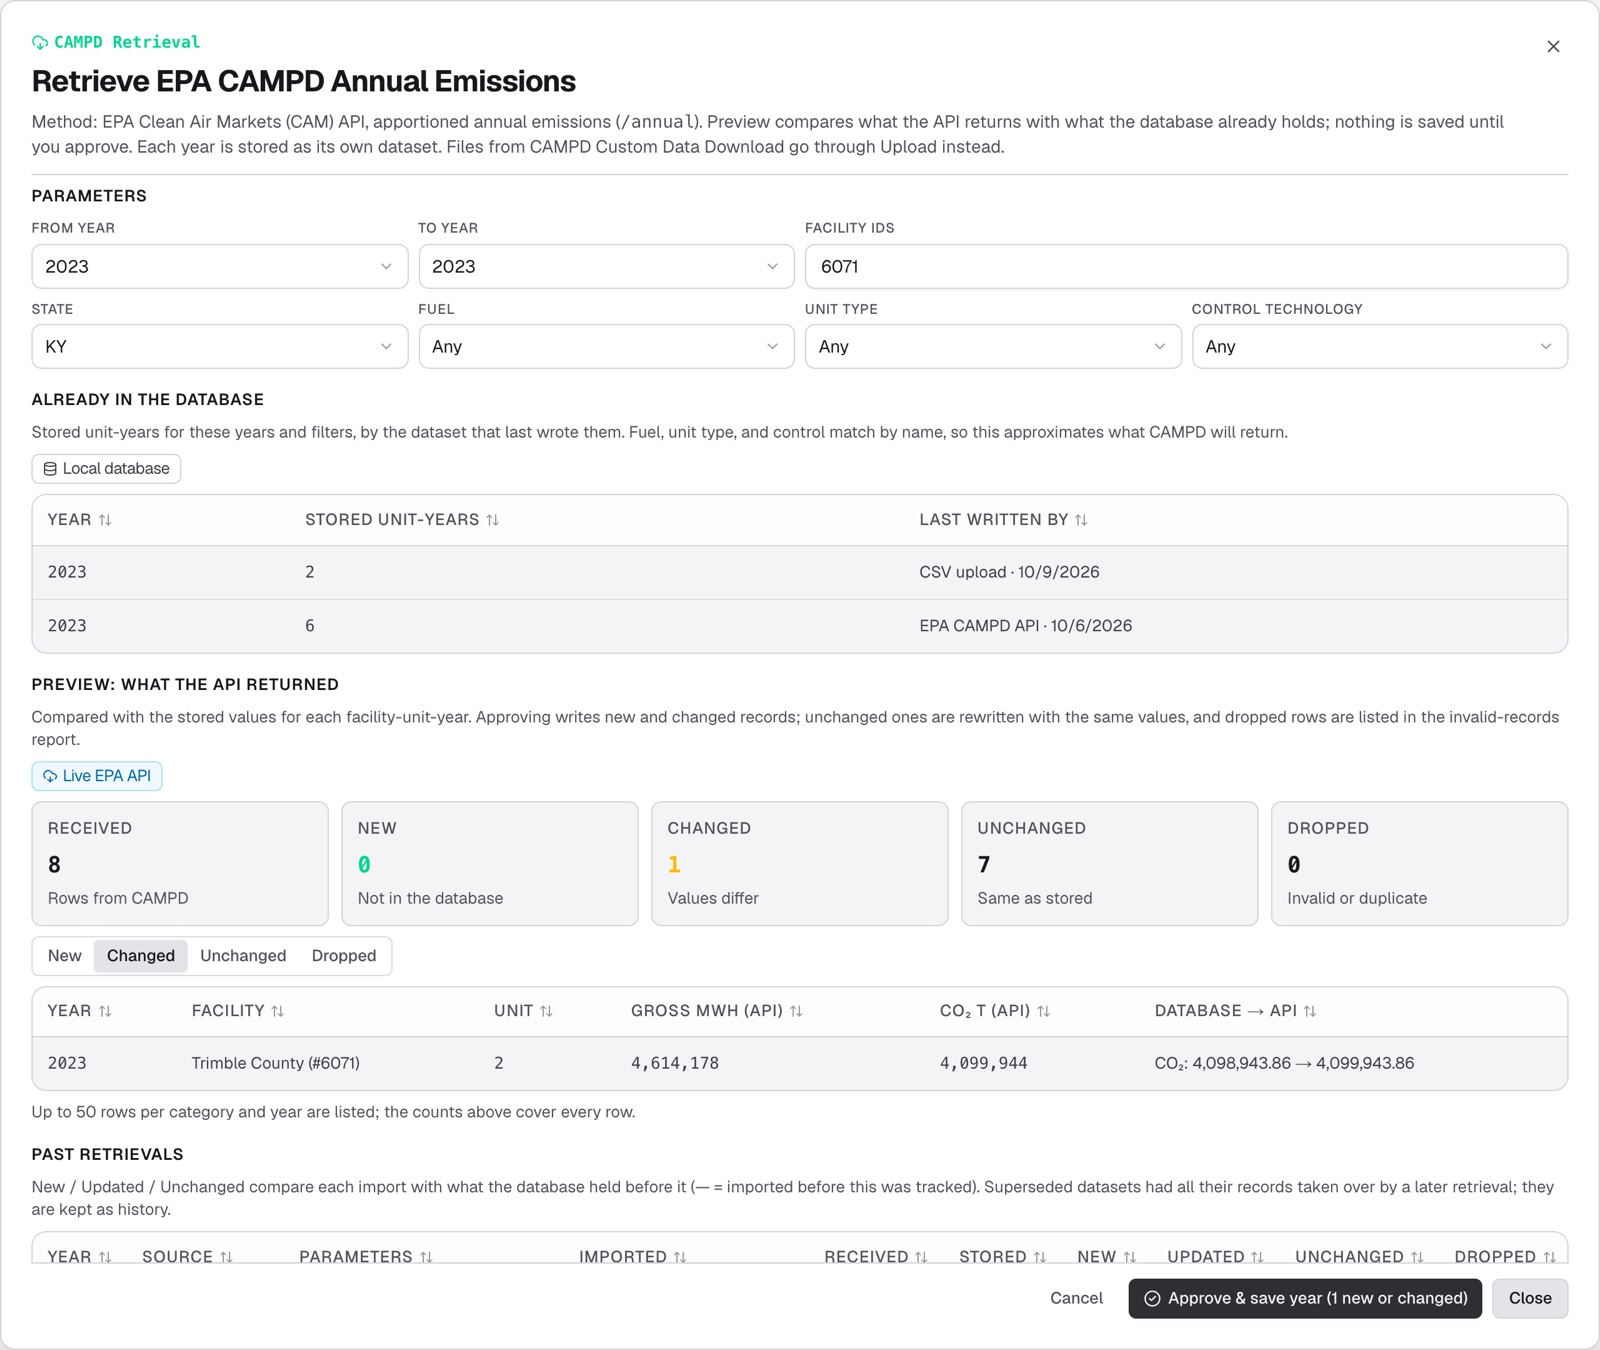
\includegraphics[width=0.92\linewidth]{retrieve-preview.jpg}
  \caption{Retrieval preview for Trimble County, 2023: the database panel (top), the API
  comparison with one changed record and its old and new value, and the approval button.}
  \label{fig:retrieve}
\end{figure}

\paragraph{How it works.} Preview and save share one fetch function,
\code{fetchCampdAnnual}, which pages through the API and validates every row with Zod. It
also removes rows that repeat a facility-unit-year, also across pages, and writes nothing.
The comparison keys every record by its natural key, facility ID, unit ID, and year, and
compares the seven stored metrics (Listing~\ref{lst:diff}). Values that differ only by
floating-point noise count as equal, so re-reading the same CAMPD figure never shows as a
change. Rows that fail validation or repeat a key are \emph{dropped}, but never silently:
saving writes them to \code{import\_issues} with the Zod message as the reason, so the
invalid-record report covers API datasets as well as uploads. The save step fetches the year
again rather than trusting the preview, and the whole year is fetched before the first write.
A network failure part-way through therefore leaves no partial dataset.

\begin{lstlisting}[language=TypeScript, caption={Record comparison (\code{src/lib/record-diff.ts}), shared by retrievals and uploads.}, label=lst:diff]
/** Natural key of a unit-year record, shared by uploads, CAMPD rows, and stored records. */
export const recordKey = (facilityId: number, unitId: string, year: number | string) =>
  `${facilityId}:${unitId}:${year}`;

/** Equal within floating-point noise (relative 1e-9). */
const same = (a: number, b: number) =>
  Math.abs(a - b) <= 1e-9 * Math.max(1, Math.abs(a), Math.abs(b));

/** New when nothing is stored; otherwise every metric that differs from the stored value. */
export function diffRecord(incoming: EmissionTotals, stored?: EmissionTotals) {
  if (!stored) return { status: "new", changes: [] };
  const changes = TOTAL_KEYS.filter((k) => !same(incoming[k], stored[k])).map(
    (field) => ({ field, database: stored[field], incoming: incoming[field] }),
  );
  return { status: changes.length ? "changed" : "unchanged", changes };
}
\end{lstlisting}

% ------------------------------------------------------------------------
\subsection{Upload validation and the data-quality report}
\label{sec:feat-upload}

The upload path implements all eleven steps of the specification. Its distinguishing property
is that nothing is lost: every row ends up either stored, or stored and flagged, or listed in
the data-quality report with a reason.

\paragraph{Validation rules.} \code{scripts/parse\_import.py} normalises each header by
lower-casing it and removing punctuation, so ``Facility ID'', \code{facility\_id}, and
\code{facilityId} all match the same alias list. It then maps the file to one of two schemas:
annual emissions (facility ID, unit ID, year, and metrics) or facilities and units (no year).
Each cell is converted by a column-specific rule (Listing~\ref{lst:parse}). Identifiers and
years must be whole numbers within bounds. Coordinates must lie within $\pm90$/$\pm180$
degrees. Metrics must be non-negative numbers, and states must be valid U.S.\ state or
territory codes. A row with any failing cell is rejected with every reason listed. A row
whose facility-unit-year already appeared earlier in the file is a duplicate and is skipped
with a reference to the first occurrence.

\begin{lstlisting}[language=Python, caption={Cell validation in \code{scripts/parse\_import.py} (abridged).}, label=lst:parse]
def parse_value(col, raw):
    """Convert a non-empty cell to its database value, or raise ValueError with the reason."""
    if col == "stateCode":
        if raw.upper() not in US_STATES:
            raise ValueError(f"Unrecognized US state or territory '{raw}'")
        return raw.upper()
    if col not in BOUNDS:
        return raw
    lo, hi, whole = BOUNDS[col]          # e.g. year: (1980, 2100, True)
    try:
        n = float(raw.replace(",", ""))
    except ValueError:
        n = math.nan
    if not math.isfinite(n):
        raise ValueError(f"Expected a number, got '{raw}'")
    if whole and not n.is_integer():
        raise ValueError(f"Expected a whole number, got '{raw}'")
    if n < lo or (hi is not None and n > hi):
        raise ValueError(f"Out of range ({lo} to {hi})" if hi is not None else f"Must be at least {lo}")
    return int(n) if whole else n
\end{lstlisting}

\paragraph{Example workflow.} The repository ships a test file,
\code{samples/annual-emissions-sample.csv}, with an identical Excel copy. It contains 25
rows of real CAMPD data for Kentucky, mostly from 2014, a year the committed database does
not cover. Five rows were altered on purpose, and one unaltered row trips a sanity rule.
Uploading it produces the report in Figure~\ref{fig:upload}:
\begin{itemize}
  \item 21 valid rows: 19 new, one changed, one unchanged;
  \item three rejected rows: a missing unit ID (row 12), the state code ``KZ'' (row 18), and a
        negative \COtwo{} mass (row 19);
  \item one duplicate: row 25 repeats row 4;
  \item one sanity flag: row 16, Robert Reid unit RT in 2014, which reported 38{,}801.9\,MMBtu of
        heat input and no \COtwo. This row is unmodified EPA data.
\end{itemize}
After approval, the Units tab filtered to origin ``File upload'' lists exactly the 21 stored
unit-years, and the invalid-record download contains the three rejected rows, the duplicate,
and the flagged record, each with its original columns.

\begin{figure}[H]
  \centering
  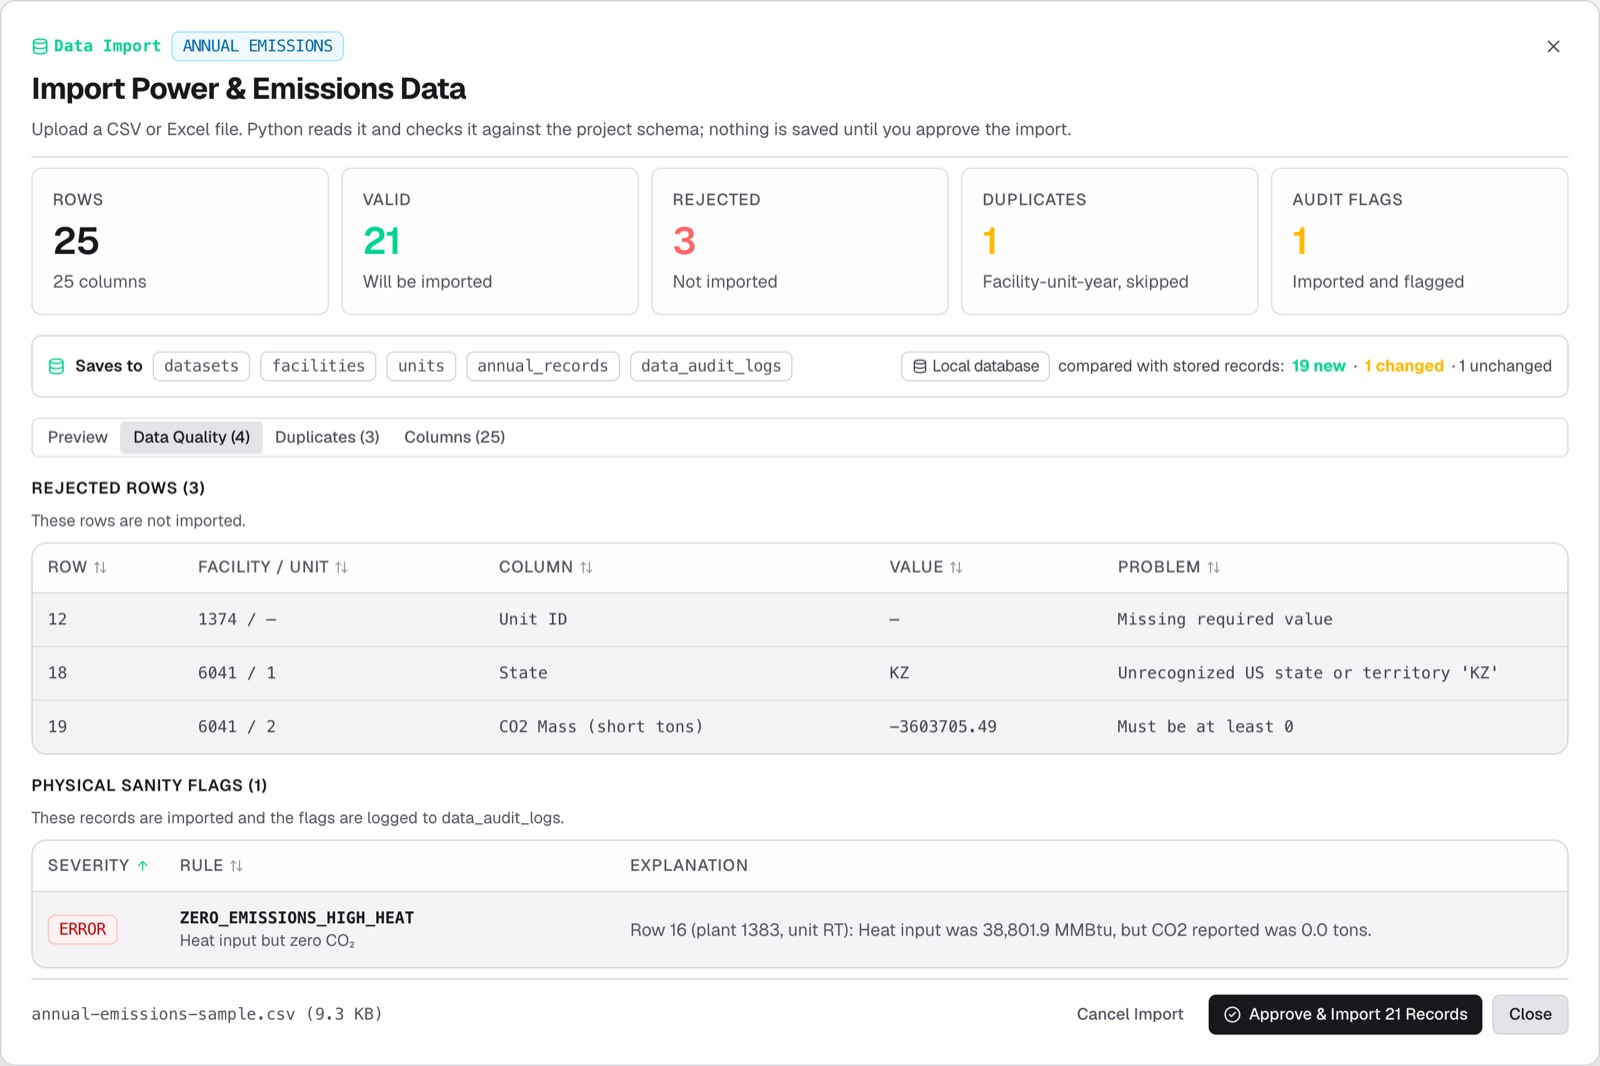
\includegraphics[width=0.92\linewidth]{upload-quality.jpg}
  \caption{Upload report for the sample file, Data Quality tab: counts, the database
  comparison, the three rejected rows with their reasons, and the physical-sanity flag.}
  \label{fig:upload}
\end{figure}

% ------------------------------------------------------------------------
\subsection{Description-based search}
\label{sec:feat-describe}

The rubric asks for a search that understands requests such as ``Find coal units in Kentucky
with high CO2 emissions.'' A large language model could translate such a sentence, but it would
make the core search depend on a network service and an API key, and its output can differ
from run to run. epaData instead uses a deterministic, rule-based parser
(\code{src/lib/describe-search.ts}). A language model is consulted only for words the parser
could not use, and only if a key is configured.

\paragraph{Algorithm.} The parser performs entity extraction rather than matching sentence
templates, so word order does not matter. It runs in two passes.

\begin{lstlisting}[language={}, caption={Outline of the description parser.}, label=lst:describe, numbers=none]
vocabulary <- filter values from the database (states, fuels, unit types, controls,
              counties, statuses) + synonyms ("scrubber" -> FGD, "gas" -> Natural Gas,
              state names -> codes) + metric, comparator, ranking, and view words

pass 1: tokens -> items
  for each position, take the LONGEST phrase (up to 6 words) found in the vocabulary
    ("west virginia" beats "virginia"; "natural gas" beats "gas")
  two-letter state codes count only in capitals ("IN", not "in")
  counties need the word "county"; names follow "owned by" / "named"
  numbers: 500,000 | 500k | 1.2M | 5e5; four-digit years
  unknown filter value within edit distance 1 (2 for long words) -> fuzzy match
  "not X" -> reported as not understood, never inverted
  anything else that is not a stopword -> not understood

pass 2: bind items
  filters -> filter values;  "units" / "plants" -> which table to show
  comparator + number -> nearest metric word, looking forward then back
     ("over 500k tons of CO2", "CO2 over 500k", "under 50 tons SO2")
  year-like numbers -> year, or year range ("since 2020", "2015-2020")
  "top / highest / most [N]" -> sort descending, keep N (default 10, or 1 if singular)
  "lowest / least / cleanest [N]" -> sort ascending;  "in each state" -> rank per state
  "high / low <metric>" without a number -> qualitative term, resolved on the server
\end{lstlisting}

Typo tolerance uses the optimal-string-alignment variant of edit distance, which counts
insertions, deletions, substitutions, and transpositions of adjacent letters, the four error
types Damerau identified as the bulk of spelling mistakes~\cite{damerau1964}. It applies only
to filter values of five letters or more, so short words are never ``corrected'' into
something else.

\paragraph{Resolving ``high'' and ``low''.} A qualitative term cannot be turned into a fixed
number in advance: 500{,}000 tons of \COtwo{} is high for a gas turbine and low for a large
coal unit. The server therefore resolves ``high $m$'' to the 75th percentile, and ``low $m$''
to the 25th percentile, of metric $m$ over the unit-years that match all the \emph{other}
filters. With $n$ matching values sorted in ascending order, $x_{(0)} \le \dots \le x_{(n-1)}$,
the threshold is the order statistic
\begin{equation}
  t_{\text{high}} = x_{(\lfloor 0.75\,(n-1) \rfloor)}, \qquad
  t_{\text{low}} = x_{(\lfloor 0.25\,(n-1) \rfloor)},
\end{equation}
obtained with a single \code{ORDER BY $m$ LIMIT 1 OFFSET $k$} query. This is the simplest of
the sample-quantile definitions compared by Hyndman and Fan~\cite{hyndman1996quantiles}:
where their common default interpolates between the two neighbouring order statistics, epaData
takes the lower one, so the threshold is always a value that occurs in the data. The threshold is rounded
to three significant figures and becomes an ordinary minimum or maximum filter, and the table
is sorted by that metric. For the rubric sentence, the 416 Kentucky coal unit-years give
$t_{\text{high}} = 2{,}660{,}000$ tons, which selects 103 unit-years (Figure~\ref{fig:describe}).
The interface states the rule next to the result, ``high = top 25\% of unit-years matching the
other filters''.

\begin{figure}[H]
  \centering
  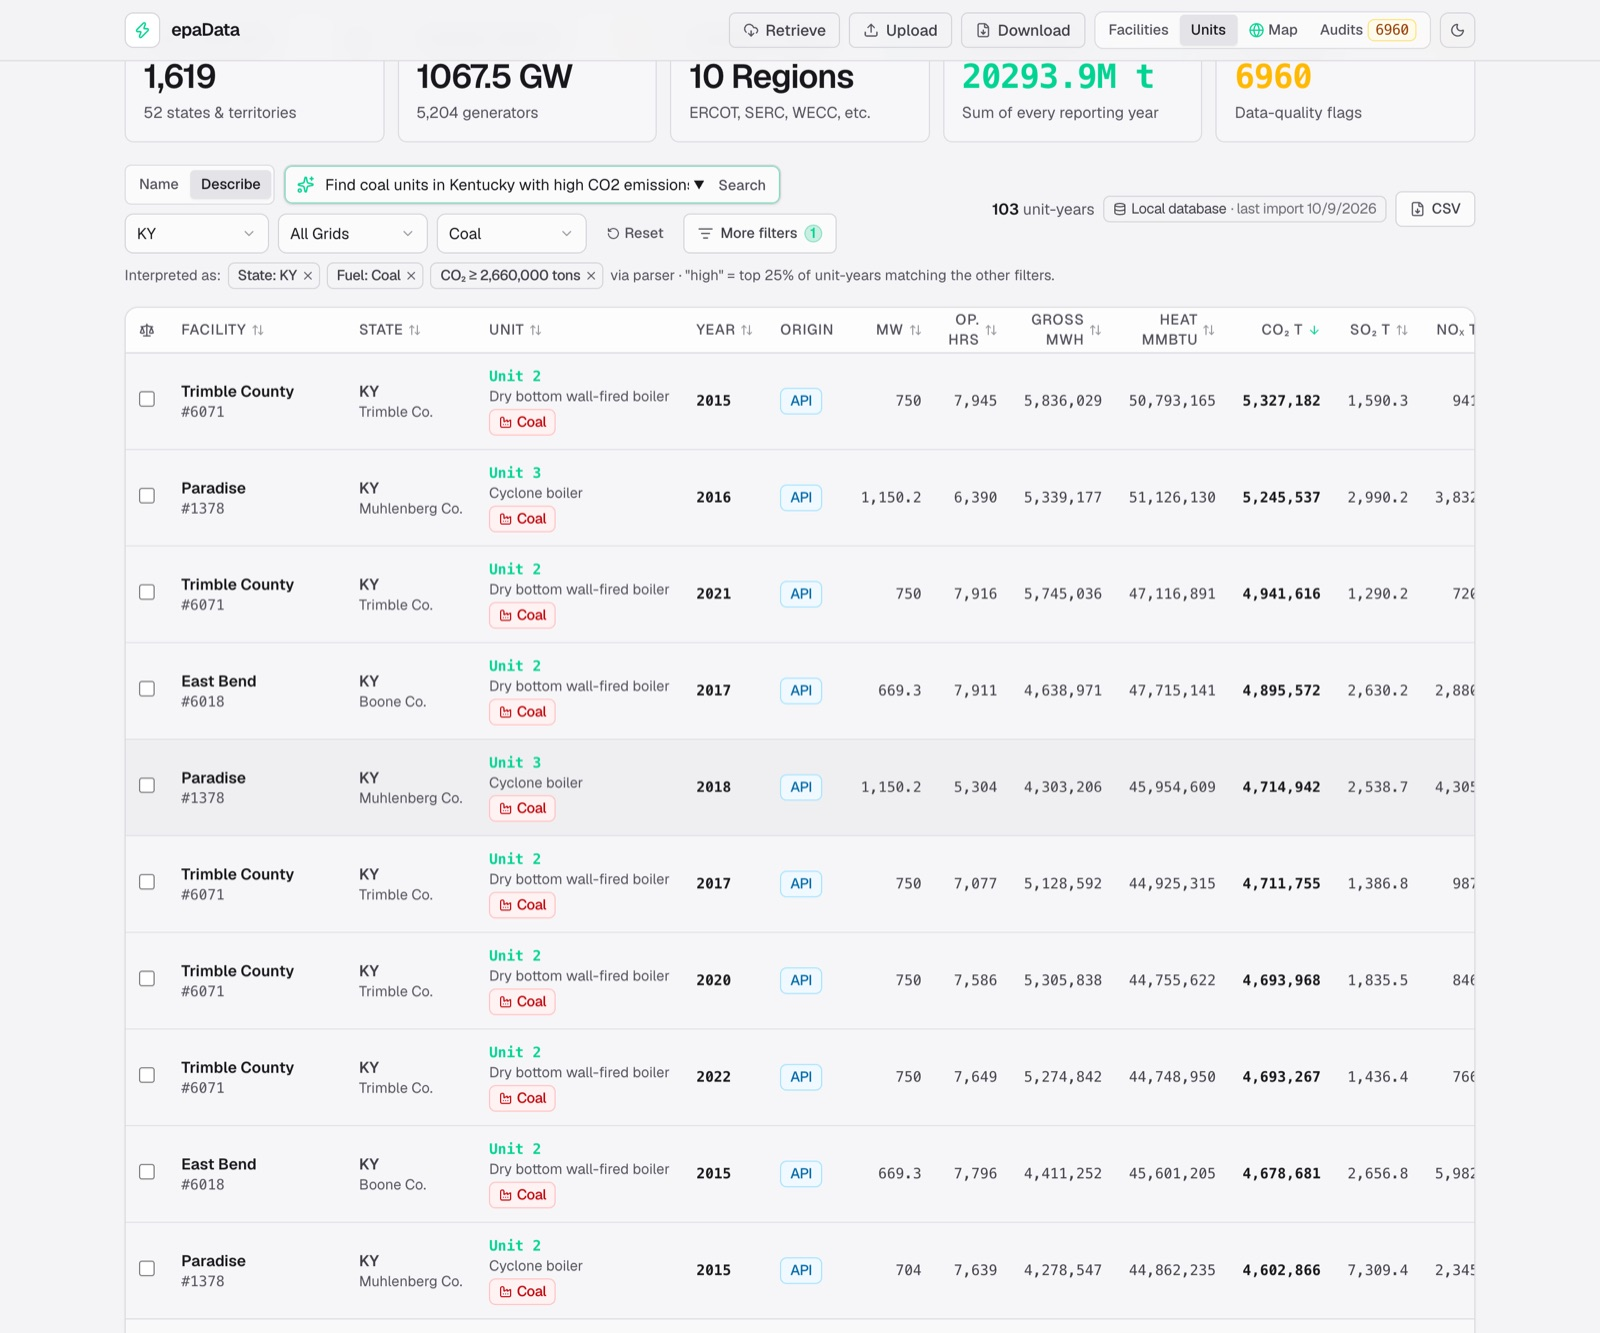
\includegraphics[width=0.92\linewidth]{describe.jpg}
  \caption{Description search on the committed database. The sentence becomes three removable
  filter chips; the note explains the threshold; 103 unit-years match, sorted by \COtwo.}
  \label{fig:describe}
\end{figure}

\paragraph{Language-model fallback.} When words remain unrecognised and
\code{OPENROUTER\_API\_KEY} is set, \code{src/server/llm-search.ts} sends the sentence, the
parser's interpretation, and the leftover words to an OpenRouter model. The request asks for
structured JSON whose schema enumerates the database's own filter values. The model may only
\emph{add} filters the parser did not set. Every returned value is re-validated with Zod
against the vocabulary, the call times out after 8 seconds, and any failure falls back to the
parser's result with a note. The key never leaves the server. The language model therefore
cannot introduce a value the database does not contain, and the search works fully without it.

\paragraph{Worked examples.} Table~\ref{tab:describe} lists ten descriptions, the filters
the parser produced, and the number of rows each returns on the committed database. None of
them needed the language model.

{\small
\begin{longtable}{@{}R{0.36\linewidth}R{0.47\linewidth}r@{}}
\caption{Description search on the committed database (parser only).}\label{tab:describe}\\
\toprule
\textbf{Description} & \textbf{Interpreted as} & \textbf{Rows}\\
\midrule\endfirsthead
\toprule
\textbf{Description} & \textbf{Interpreted as} & \textbf{Rows}\\
\midrule\endhead
Find coal units in Kentucky with high CO2 emissions. & Units; KY; Coal; \COtwo{} $\ge$ 2{,}660{,}000; sort \COtwo{}$\downarrow$ & 103\\
coal units in Kentucky in 2025 with CO2 over 500,000 tons & Units; KY; Coal; 2025; \COtwo{} $\ge$ 500{,}000 & 25\\
top CO2-emitting facility in each state in 2024 & Facilities; 2024; first 1 per state by \COtwo{}$\downarrow$ & 51\\
top 20 units by gross generation in 2025 & Units; 2025; first 20 by gross load$\downarrow$ & 20\\
units with the lowest NOx emissions in 2025 & Units; 2025; first 10 by \NOx{}$\uparrow$ & 10\\
gas units in TX under 50 tons SO2 & Units; TX; Natural Gas; \SOtwo{} $\le$ 50 & 4{,}374\\
operating gas units in Texas with low NOx since 2020 & Units; TX; Natural Gas; Operating; year $\ge$ 2020; \NOx{} $\le$ 8.46; sort \NOx{}$\uparrow$ & 670\\
plants owned by Duke Energy with scrubbers & Facilities; text ``Duke Energy''; \SOtwo{} control FGD & 11\\
units in IN with heat input above 5M MMBtu in 2025 & Units; IN; 2025; heat input $\ge$ 5{,}000{,}000; sort heat input$\downarrow$ & 42\\
Kentuky coal units that are not retired & Units; KY (typo corrected); Coal; \emph{not understood: ``not retired''} & 416\\
\bottomrule
\end{longtable}}

% ------------------------------------------------------------------------
\subsection{Multi-constraint search and ranking in SQL}
\label{sec:feat-ranking}

The specification's example, ``coal-fired units in Kentucky in 2025 with annual \COtwo{}
emissions greater than 500{,}000 short tons'', is a conjunction of three kinds of condition:
on the facility (state), on the unit (fuel), and on the unit-year (year and \COtwo). The query
builder keeps one function per kind and combines their output with AND
(Figure~\ref{fig:multi}). Fuel, unit-type, and control filters match by substring, because
CAMPD stores combined values such as ``Coal, Pipeline Natural Gas'' or
``Wet Lime FGD|Wet Limestone''. Operating status matches by prefix, so that ``Retired'' does
not also match ``Operating (Retired 04/15/2016)''.

\begin{figure}[H]
  \centering
  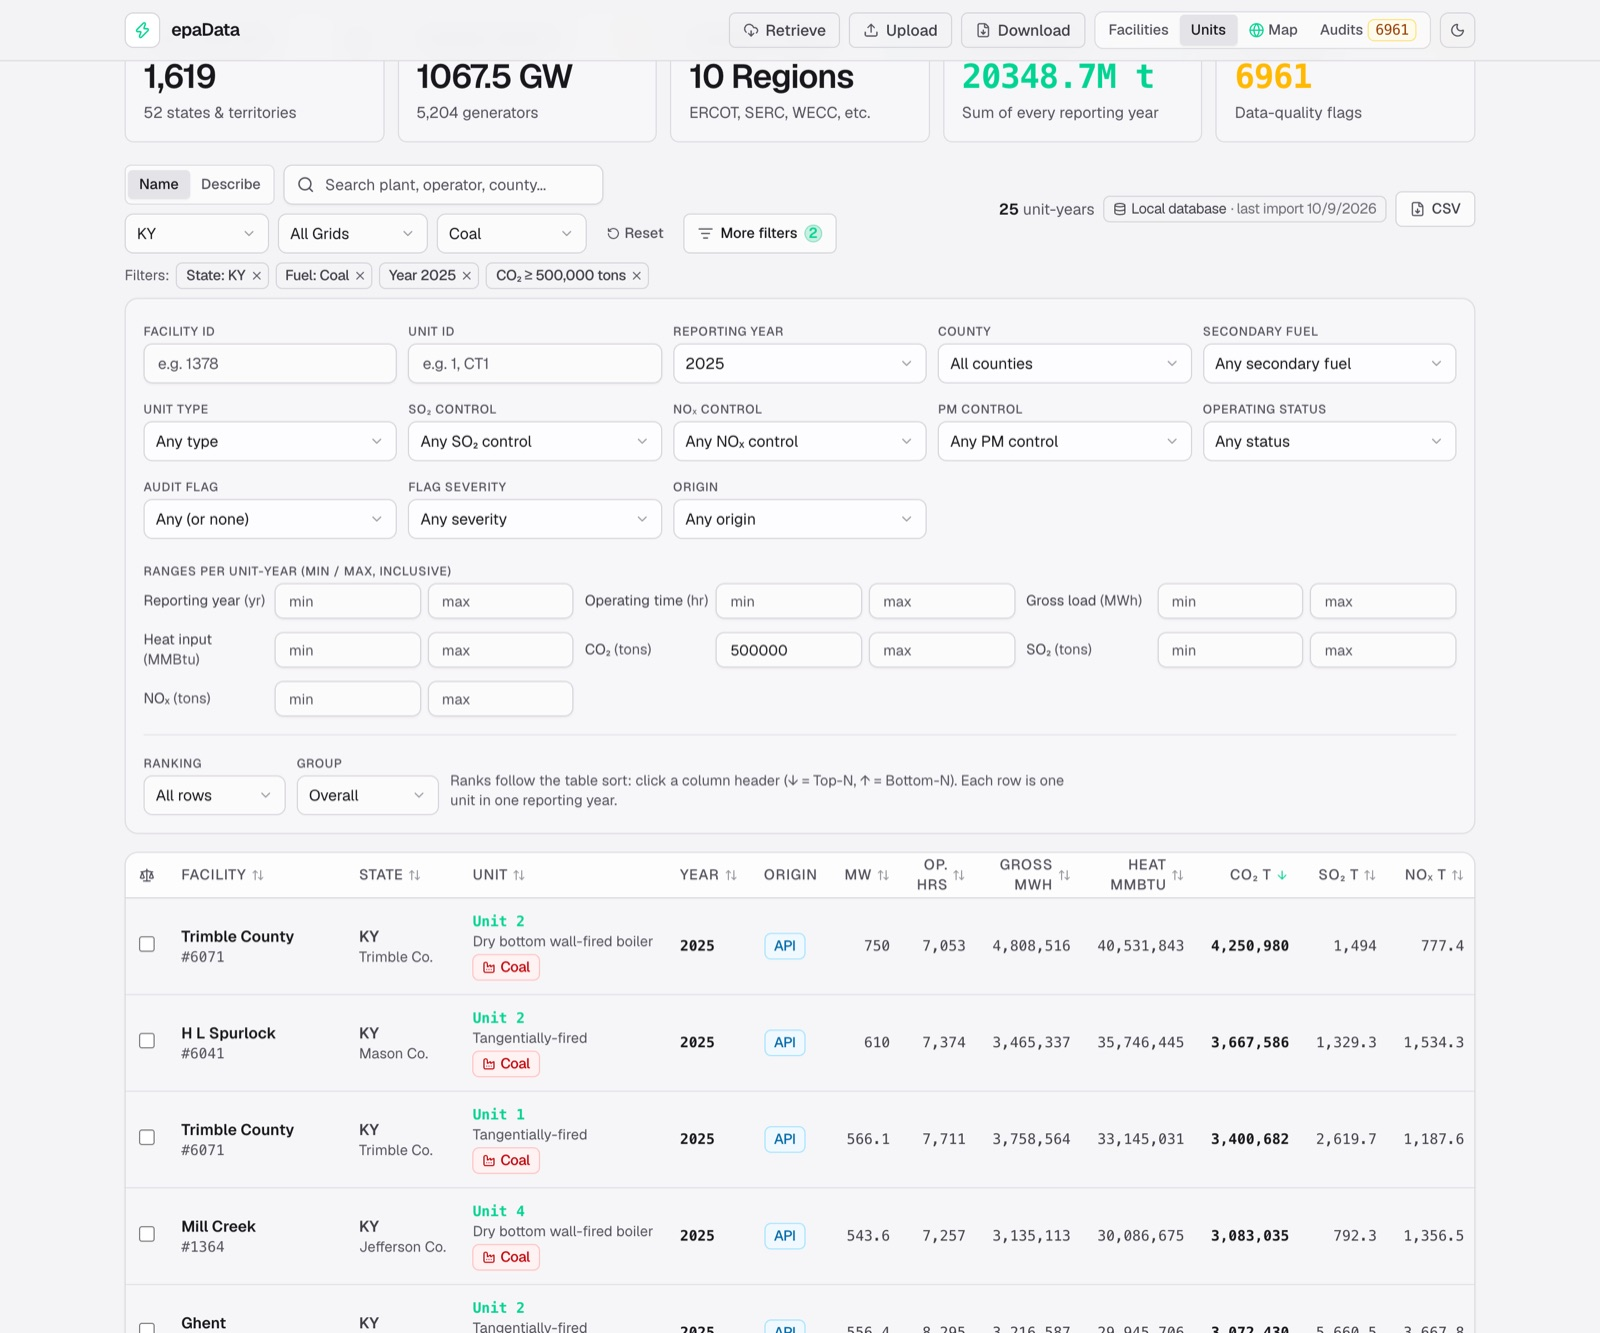
\includegraphics[width=0.92\linewidth]{units-multi.jpg}
  \caption{Multi-constraint search: KY, Coal, 2025, \COtwo{} $\ge$ 500{,}000\,t. The chips, the
  open \emph{More filters} panel with its range inputs, and the first rows of the 25 results.}
  \label{fig:multi}
\end{figure}

Ranking is implemented with a window function. Listing~\ref{lst:rank} shows, simplified, the
SQL that \code{rankedUnitYears} generates for ``the highest-\COtwo{} coal unit-year in each
state in 2025''. The inner query numbers the matching rows in sort order, restarting the
numbering for each state when ranking per state. The outer query keeps the first $N$ ranks.
The same subquery feeds the page of rows, the total count, and the CSV export, so all three
always agree. \code{IS NULL} in the ordering puts missing values last in either direction,
and the record ID breaks ties so that paging is stable.

\begin{lstlisting}[style=sql, caption={Ranking query generated for a per-state top-1 search (simplified).}, label=lst:rank]
SELECT * FROM (
  SELECT ar.id, f.name, f.state_code, u.unit_id, ar.year, ar.co2_mass_tons, d.source AS origin,
         ROW_NUMBER() OVER (
           PARTITION BY f.state_code                      -- only when ranking per state
           ORDER BY ar.co2_mass_tons IS NULL, ar.co2_mass_tons DESC, ar.id
         ) AS rank
  FROM annual_records ar
  JOIN units u       ON ar.unit_internal_id = u.id
  JOIN facilities f  ON ar.facility_id = f.id
  LEFT JOIN datasets d ON ar.dataset_id = d.id
  WHERE lower(u.primary_fuel) LIKE '%coal%'           -- unit condition (contains)
    AND ar.year = 2025                                -- record conditions
) AS ranked
WHERE rank <= 1                                       -- keep the first N
ORDER BY state_code, rank
LIMIT 25 OFFSET 0;                                    -- one page
\end{lstlisting}

The Facilities view ranks plants by totals computed with correlated subqueries, for example
the sum of \COtwo{} over a facility's records in the selected year. Unit and unit-year filters
keep a facility if at least one of its unit-years matches, expressed as an \code{IN} subquery
so that the facility row is not duplicated. Figure~\ref{fig:ranking} shows the per-state
ranking for 2024.

\begin{figure}[H]
  \centering
  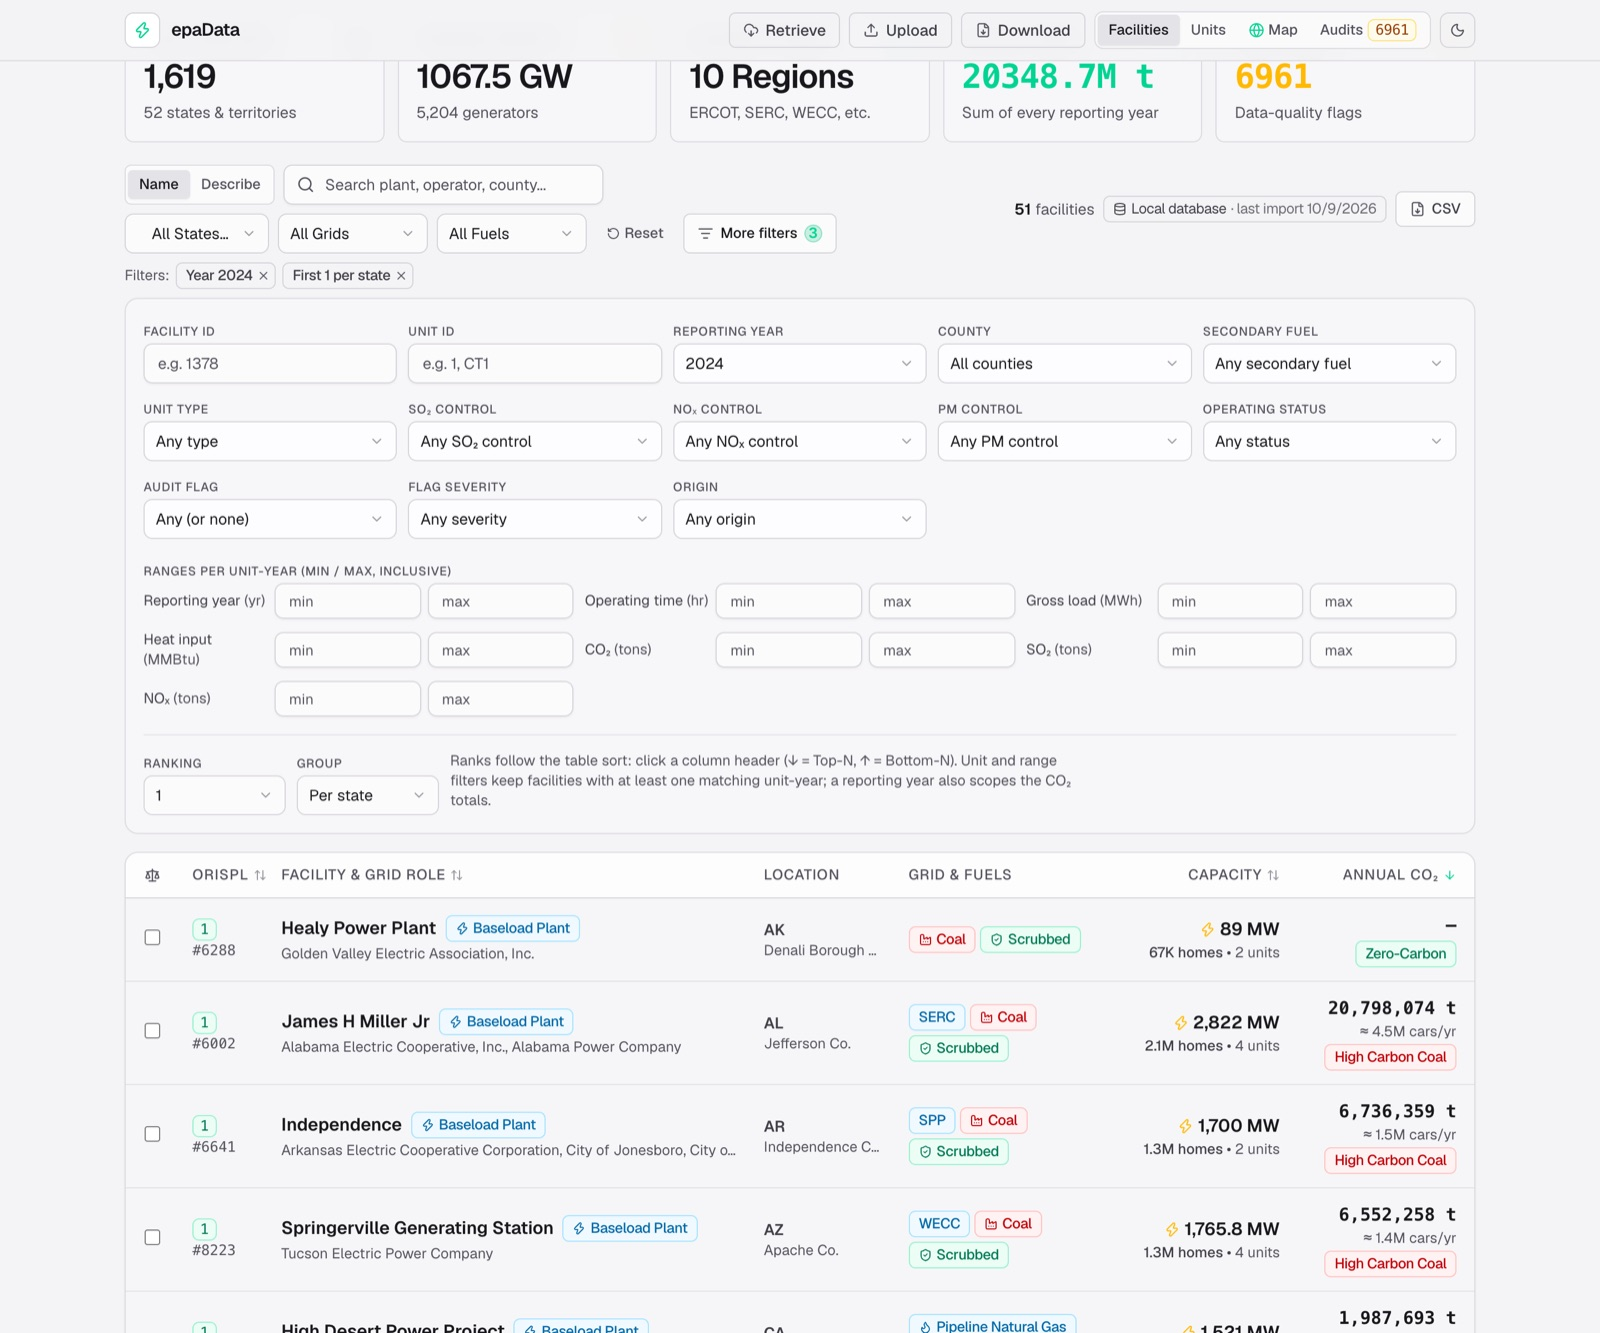
\includegraphics[width=0.92\linewidth]{ranking.jpg}
  \caption{Group-and-rank: the top \COtwo-emitting facility in each state in 2024 (51 rows).}
  \label{fig:ranking}
\end{figure}

% ------------------------------------------------------------------------
\subsection{Physical-sanity audits}
\label{sec:feat-audits}

Validation catches values that are malformed; it cannot catch values that are well-formed but
physically implausible. epaData therefore applies three rules to every annual record it
writes, whatever its source. Let $H$ be heat input (MMBtu), $G$ gross load (MWh), $T$
operating time (hours), and $C$ the \COtwo{} mass (short tons). The derived rates stored with
each record are
\begin{equation}
  \text{heat rate} = \frac{H}{G}\ \ \text{MMBtu/MWh}, \qquad
  \text{\COtwo{} intensity} = \frac{2000\,C}{G}\ \ \text{lb/MWh},
\end{equation}
both undefined (stored as \code{NULL}) when $G = 0$. The rules, with thresholds defined once
in \code{AUDIT\_THRESHOLDS}, are:
\begin{align}
  \texttt{ZERO\_EMISSIONS\_HIGH\_HEAT} \;(\text{ERROR}):&\quad H > 1000 \ \wedge\ C = 0,\\
  \texttt{PHANTOM\_GENERATION} \;(\text{ERROR}):&\quad G > 0 \ \wedge\ T = 0,\\
  \texttt{EXTREME\_HEAT\_RATE} \;(\text{WARN}):&\quad H/G < 5 \ \vee\ H/G > 25.
\end{align}
The first rule reflects that burning fossil fuel always produces \COtwo. The second, that a
unit cannot generate without running. The third bounds the heat rate by the thermodynamic
range of real fossil plants, which typically lie between about 6.5\,MMBtu/MWh (modern
combined-cycle units) and 15--18\,MMBtu/MWh (old peaking units). Flagged records are kept, not discarded: they appear in the
Audits tab, in the unit and facility dialogs, and in the invalid-record export. In the
committed database the rules flag 6{,}960 records: 855 extreme heat rates (WARN) and 6{,}105
zero-\COtwo{} records (ERROR). Most of the latter are gas- and oil-fired units, and 2{,}637 of
them also report no gross load. In these records CAMPD gives heat input but no \COtwo{} mass,
which epaData stores as zero. The rule therefore cannot tell a \COtwo{} value that was not
reported from one reported as zero, and many of these flags mean ``\COtwo{} not reported''
rather than a measurement error (Section~\ref{sec:limitations}).

% ------------------------------------------------------------------------
\subsection{Provenance and export}
\label{sec:feat-provenance}

Every number in epaData can be traced. The unit dialog (Figure~\ref{fig:unit}) lists each
reporting year with the dataset that wrote it. The Units table shows the same information
as an \emph{Origin} badge, and the \emph{Origin} filter restricts any search to API or
uploaded records. The Download dialog (Figure~\ref{fig:download}) exports the provenance
table itself: one row per dataset with its source, date, query parameters as JSON, file name,
and the received, stored, flagged, new, updated, unchanged, and dropped counts. Unit-year
exports include \code{dataset\_id}, \code{origin}, and \code{dataset\_imported\_at} for every
row. All exports are written by one CSV function that quotes fields according to
RFC~4180.

\begin{figure}[H]
  \centering
  \begin{minipage}[t]{0.55\linewidth}
    \centering
    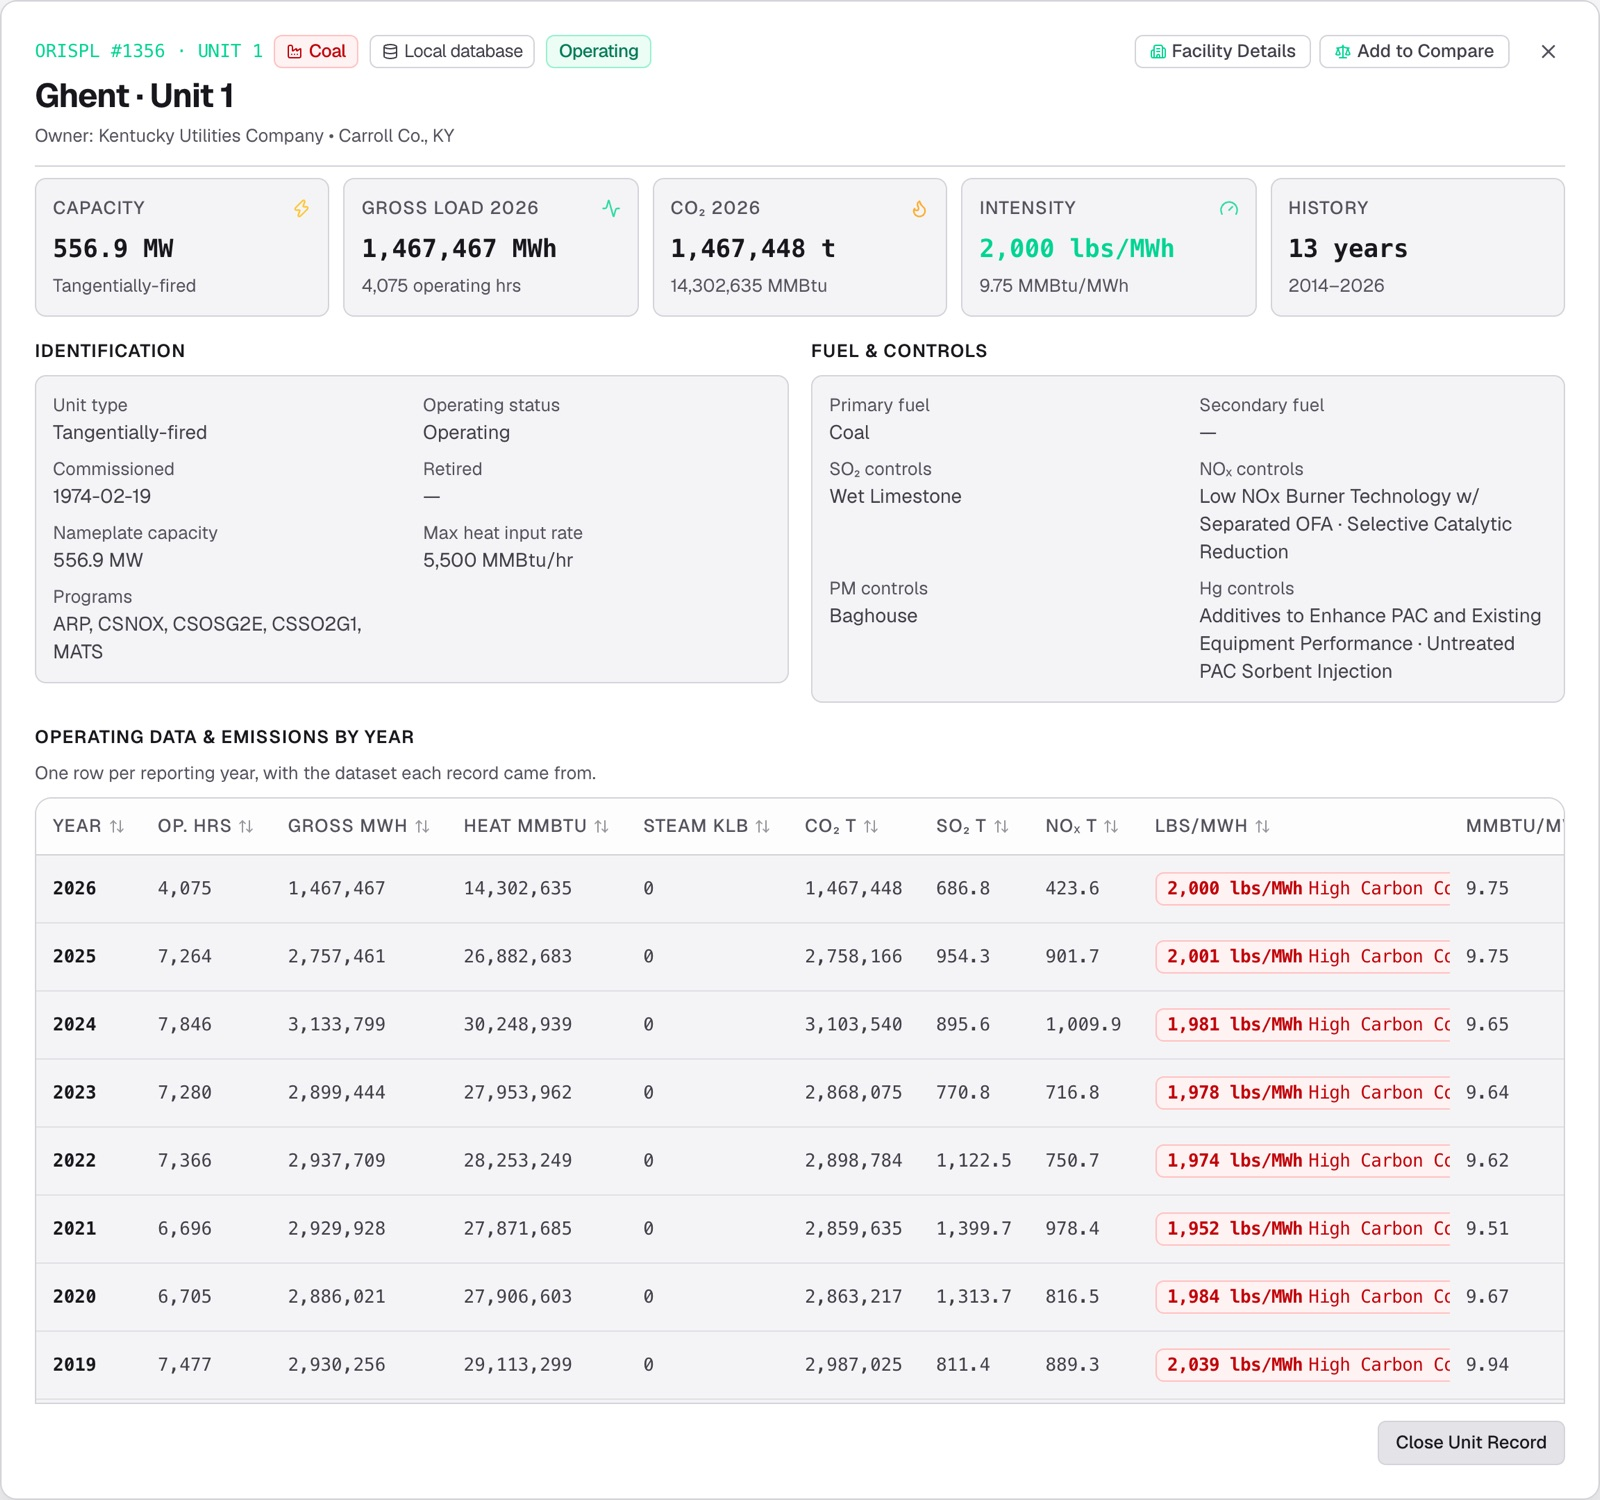
\includegraphics[width=\linewidth]{unit-detail.jpg}
    \caption{Unit dialog: Ghent unit 1 after the sample upload, with 13 reporting years (2014 from the upload, 2015--2026 from the API).}
    \label{fig:unit}
  \end{minipage}\hfill
  \begin{minipage}[t]{0.42\linewidth}
    \centering
    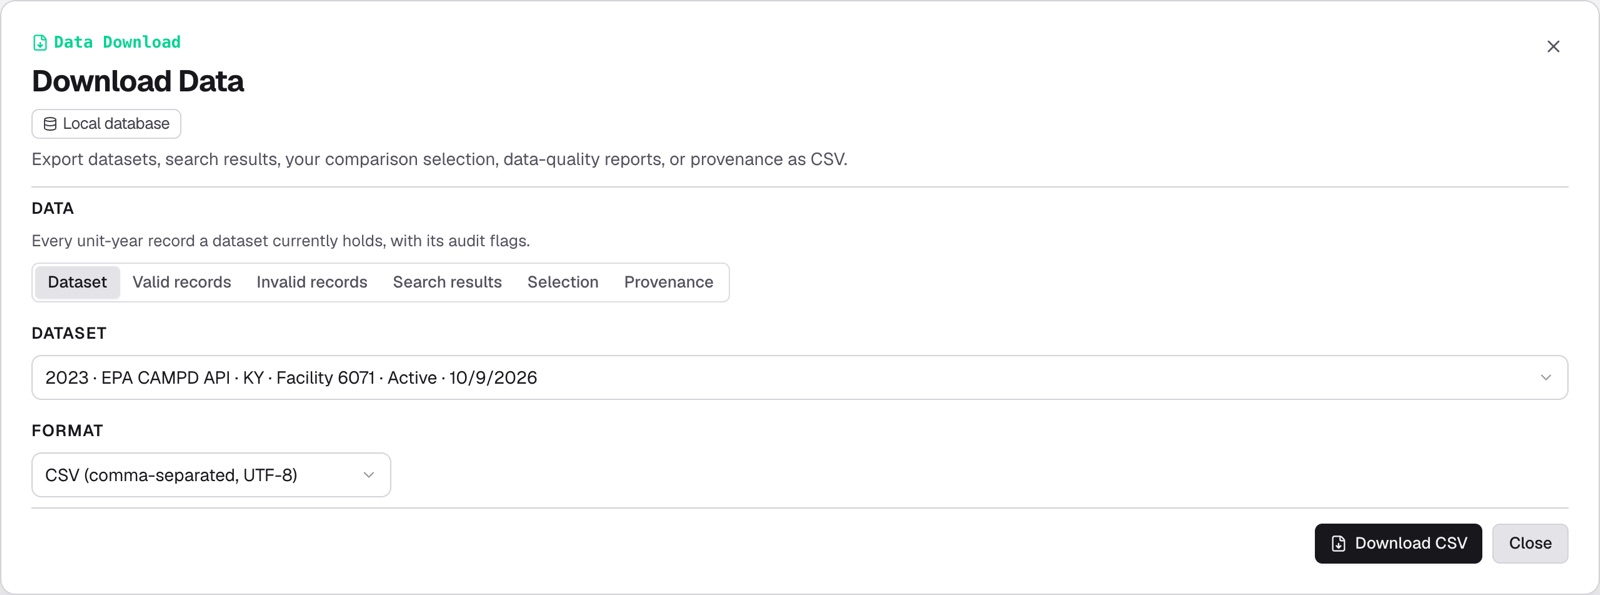
\includegraphics[width=\linewidth]{download.jpg}
    \caption{Download dialog: data type, dataset, filters, and format.}
    \label{fig:download}
  \end{minipage}
\end{figure}

% ------------------------------------------------------------------------
\section{Testing and results}
\label{sec:testing}

\subsection{Approach}

The system was tested at four levels.
\begin{enumerate}
  \item \textbf{Static checks.} \code{npm run validate} runs Prettier, ESLint, the TypeScript
        compiler in strict mode, the unit tests, and a production build; the project was
        kept passing after every development stage. Type checking catches a large class of
        errors early, because database rows, procedure inputs, and component props share types.
  \item \textbf{Unit tests.} 39 tests with Node's built-in test runner cover the logic in
        \code{src/lib}, which has no database or network access, and the Python upload parser,
        which the tests run as a subprocess on generated and committed files.
  \item \textbf{Acceptance tests against hand-written SQL.} For each search in the
        specification, the result of the application, through its HTTP API, was compared
        with an independent SQL query written directly against the database.
  \item \textbf{End-to-end tests on database copies.} The upload, retrieval, and export flows
        were exercised over HTTP, and the user interface was driven through a scripted headless
        browser, which also produced the screenshots in this report. These runs used copies of
        \code{db.sqlite}, so the committed data stayed unchanged.
\end{enumerate}

\subsection{Unit tests}

Table~\ref{tab:unittests} summarises the unit tests by file. Each test contains several
assertions; the description-search tests, for example, check about sixty phrasings, including
three word orders of the same request that must yield identical filters.

\begin{table}[H]
\centering\small
\caption{Unit tests (\code{npm test}: 39 tests, all passing).}
\label{tab:unittests}
\begin{tabularx}{\linewidth}{@{}>{\raggedright\arraybackslash}p{0.27\linewidth}cL@{}}
\toprule
\textbf{File} & \textbf{Tests} & \textbf{What is checked}\\
\midrule
\code{describe-search.test.ts} & 12 & Rubric and specification sentences; word-order permutations; ranges, units of measure, and \emph{between}; top-$N$, bottom-$N$, and per-state ranking; years and year ranges; synonyms, controls, and statuses; state names, codes, and ambiguous lower-case codes; owner names; typos; negation and unknown words; number formats.\\
\code{domain-utils.test.ts} & 13 & Emissions arithmetic with missing generation; fuel metadata; control rules; reporting-period dates and EPA's published-through quarter; yearly roll-ups; retrieval filters; explorer state round-trip through the URL and rejection of invalid parameters; option splitting; sorting.\\
\code{data-import.test.ts} & 7 & Extension and size checks; rejected rows, duplicates, and sanity flags on a generated file; column mapping; refusal of files without IDs; Excel reading; a real CAMPD facility file (skipped when absent); the committed sample files (Section~\ref{sec:feat-upload}).\\
\code{record-diff.test.ts} & 4 & New, unchanged (including floating-point noise), and changed records with both values; counting and natural keys.\\
\code{csv.test.ts} & 3 & RFC~4180 quoting of commas, quotes, and line breaks; CRLF line endings; export URLs.\\
\bottomrule
\end{tabularx}
\end{table}

\subsection{Representative test cases}

Table~\ref{tab:cases} lists representative acceptance and end-to-end cases. The expected value
comes from an independent source, usually a hand-written SQL query or the documented contents
of the sample file, and the actual value from the application. All counts refer to the
committed database unless stated otherwise.

{\small
\begin{longtable}{@{}R{0.36\linewidth}R{0.3\linewidth}R{0.2\linewidth}c@{}}
\caption{Representative test cases.}\label{tab:cases}\\
\toprule
\textbf{Input} & \textbf{Expected (source)} & \textbf{Actual} & \textbf{Pass}\\
\midrule\endfirsthead
\toprule
\textbf{Input} & \textbf{Expected (source)} & \textbf{Actual} & \textbf{Pass}\\
\midrule\endhead
Units: KY, Coal, 2025, \COtwo{} $\ge$ 500{,}000 & 25 unit-years (SQL) & 25 & \checkmark\\
Facilities: same filters & 8 facilities (SQL) & 8 & \checkmark\\
Facilities: 2024, top 1 per state by \COtwo & 51, one per state with 2024 data (SQL) & 51 & \checkmark\\
Units: facility 3, unit 1, 2015--2025 & 11 years (SQL) & 11 & \checkmark\\
Units: operating status ``Retired'' & 31, prefix match (SQL) & 31 & \checkmark\\
Describe: ``Find coal units in Kentucky with high CO2 emissions.'' & P75 of 416 values = 2{,}656{,}019 $\to$ 2{,}660{,}000; 103 rows (SQL) & 2{,}660{,}000; 103 rows & \checkmark\\
Describe: same request in three word orders & Identical filters & Identical & \checkmark\\
Describe: ``Kentuky coal units that are not retired'' & KY, Coal; ``not retired'' reported & As expected & \checkmark\\
CSV export of the description search & 103 data rows & 103 & \checkmark\\
2025 dataset (CAMPD API) & 3{,}989 records, 420 flagged (SQL) & 3{,}989; 420 & \checkmark\\
Upload the sample file (\code{samples/}, CSV) & 25 rows: 21 valid (19 new, 1 changed, 1 unchanged), 3 rejected, 1 duplicate, 1 flag (sample README) & As expected & \checkmark\\
Upload the Excel copy & Same report as the CSV & Same & \checkmark\\
Approve the sample upload & 21 records stored; 4 issues; Origin = Upload lists 21 & 21; 4; 21 & \checkmark\\
Upload the sample again & 21 unchanged, 0 new & 21; 0 & \checkmark\\
Retrieve KY, facility 6071, 2023 after the upload & 8 received, 1 changed (\COtwo{} restored), 7 unchanged & As expected & \checkmark\\
Retrieve preview, then cancel & No dataset written & Dataset count unchanged & \checkmark\\
Upload a \code{.pdf} file / an empty file & Rejected before parsing & Rejected with reason & \checkmark\\
Search the client and server bundles for the EPA key & 0 occurrences & 0 & \checkmark\\
\bottomrule
\end{longtable}}

\subsection{Performance}

Response times were measured on a laptop (Apple silicon) against a production build, as the
median of three requests after one warm-up. Table~\ref{tab:perf} shows the results.

\begin{table}[H]
\centering\small
\caption{Measured response times on the full database (50{,}947 unit-years).}
\label{tab:perf}
\begin{tabularx}{\linewidth}{@{}Lr@{}}
\toprule
\textbf{Operation} & \textbf{Time}\\
\midrule
Multi-constraint unit search (KY, Coal, 2025, \COtwo{} $\ge$ 500{,}000), one page & 5\,ms\\
Description search (parse and percentile threshold) & 12\,ms\\
Facilities, default view, one page & 60\,ms\\
Units, no filters (count over all 50{,}947 rows), one page & 210\,ms\\
Top facility per state in 2024, \emph{before} the \code{(facility\_id, year)} index & 9{,}500\,ms\\
Top facility per state in 2024, \emph{after} the index & 22\,ms\\
CSV export of all 50{,}947 unit-years & 1.4\,s\\
Preview of a full year from the EPA API (3{,}989 rows, 8 pages) & 2.3\,s\\
\bottomrule
\end{tabularx}
\end{table}

The two ranking rows record a defect found during testing for this report. Any facility-level
query with a year filter took 4--10 seconds, while the same query without a year took 90\,ms.
SQLite's query plan showed why: the per-facility totals are correlated subqueries of the form
\code{WHERE facility\_id = ? AND year = ?}, and with only single-column statistics the planner
chose the \code{(year, co2\_mass\_tons)} index. It thus scanned all four thousand records of the
year once for each of the 1{,}619 facilities. A composite index on \code{(facility\_id, year)},
added as migration~0005, lets the planner match both conditions; the query became over four
hundred times faster with identical results.

\subsection{Known issues}

\begin{itemize}
  \item \textbf{Missing \COtwo{} is stored as zero.} CAMPD leaves \COtwo{} mass empty for some
        records that do report heat input. Metric columns are non-null with a default of zero,
        so these records trip the zero-emissions rule; most of the 6{,}105 ERROR flags are of
        this kind (Section~\ref{sec:feat-audits}).
  \item \textbf{Compare dialog label.} The comparison dialog labels CAMPD's gross load as
        ``Net Generation''. The value is gross load, as everywhere else in the application.
  \item \textbf{Facilities without coordinates.} 37 of the 1{,}619 facilities have no latitude
        or longitude and therefore do not appear on the map; they appear in every other view.
  \item \textbf{Dialog accessibility.} The shared dialog component closes on Escape and on an
        outside click, but does not declare \code{role="dialog"} or trap keyboard focus, so
        screen readers do not announce it as a dialog.
  \item \textbf{Language-model fallback.} The failure paths (no key, invalid key, timeout) were
        tested; the success path depends on an OpenRouter key that was not available during
        testing.
  \item \textbf{Duplicates tab.} The upload report's Duplicates tab lists both repeats within
        the file and rows that already exist in the database (``will update'' or
        ``unchanged''). This is intended, but its count differs from the Duplicates tile, which
        counts only repeats within the file.
\end{itemize}

\subsection{Does the project meet its objectives?}

Table~\ref{tab:objectives} assesses each Phase~1 objective from Section~\ref{sec:description}.

\begin{table}[H]
\centering\small
\caption{Assessment of the Phase 1 objectives.}
\label{tab:objectives}
\begin{tabularx}{\linewidth}{@{}p{0.7cm}>{\raggedright\arraybackslash}p{0.26\linewidth}p{1.4cm}L@{}}
\toprule
& \textbf{Objective} & \textbf{Verdict} & \textbf{Evidence}\\
\midrule
O1 & Web system with front end and database & Met & Sections~\ref{sec:functions} and~\ref{sec:design}.\\
O2 & Routes, templates, forms, interactive components & Met & With Next.js and React in place of Flask and Jinja (Section~\ref{sec:discussion}).\\
O3 & Relational database with SQLite and an ORM & Met & Six tables, keys, cascades, 14 indexes; Drizzle in place of SQLAlchemy.\\
O4 & Retrieve public data or import files & Met & CAM API retrieval with preview; CSV and Excel upload.\\
O5 & Validate, clean, transform, store & Met & Upload and retrieval validation; issues kept; sanity audits.\\
O6 & Search, filter, sort, paginate & Met & Basic, multi-constraint, ranking, and description search; all results sortable and paginated; Table~\ref{tab:cases}.\\
O7 & Export data and results & Met & Six CSV export types.\\
O11 & Test and deploy & Partly met & Tested as described above. Runs locally from the README; not deployed to a public host.\\
O12 & Document sources, assumptions, equations, units, limitations & Met & README, \code{DATABASE\_BREAKDOWN.md}, this report.\\
\bottomrule
\end{tabularx}
\end{table}

In summary, every Phase~1 data-management requirement is implemented and tested, and every
specification example returns the result an independent SQL query gives. The one objective
only partly met is deployment, which was deliberately limited to a local installation.

% ------------------------------------------------------------------------
\section{Discussion}
\label{sec:discussion}

\subsection{Which techniques and tools worked best for which tasks}

\paragraph{SQL for search and ranking.} Ranking, the specification's top-$N$, bottom-$N$, and
group-and-rank searches, is a natural fit for SQL window functions. Computing ranks in the
database, rather than sorting fetched rows in TypeScript, means that pagination, the total
count, and the CSV export are all derived from one ranked subquery and cannot disagree. Only
one page of rows ever leaves the database. The same reasoning applies to the percentile
thresholds of the description search: a single \code{ORDER BY \ldots{} LIMIT 1 OFFSET $k$}
query is both simpler and faster than loading the values.

\paragraph{Python for reading files.} The specification requires uploaded files to be read
with Python, and the requirement proved sensible. Python's \code{csv} module and
\code{openpyxl} handle encodings, byte-order marks, quoted fields, Excel dates, and typed
cells with little code. Running the parser as a subprocess with a JSON interface kept the
boundary simple. The Python side decides what a valid row is, and the TypeScript side decides
what to do with valid rows.

\paragraph{TypeScript for the shared write path.} The most valuable structural decision was to
give retrieval, upload, and the command-line sync one write path. Diffing against stored
records, upserting, deriving rates, auditing, and logging issues are implemented once in
\code{ingest.ts}. When the database-versus-API comparison was added, it worked for uploads at
the same time, and a fix to the audit rules applies to every source. Static types made this
refactoring safe: changing the shape of a record type surfaced every affected call site at
compile time.

\paragraph{Zod at every boundary.} Every value that enters the server from outside, whether
procedure inputs, CAMPD rows, environment variables, or language-model output, is parsed with a
Zod schema before use. Malformed input therefore fails at the boundary with a readable message
rather than deep inside a query.

\subsection{Important technical choices and alternatives}

\paragraph{Next.js, tRPC, and Drizzle instead of Flask, Jinja, and SQLAlchemy.} The course
suggests a Flask application with Jinja templates and SQLAlchemy; the team's Phase~1
proposal specified a Next.js stack instead. The motivation was interactivity: the explorer
updates results as filters change, keeps state in the URL, and opens nested dialogs, all of
which would need a separate JavaScript layer on top of server-rendered Jinja pages. With one
language and tRPC, the server's procedure signatures are the client's API, so a renamed filter
or a changed result field is a compile error rather than a runtime bug. The cost is a second
language for file parsing and a subprocess boundary. Each element of the suggested stack still
has a direct counterpart: route handlers and procedures for Flask routes, React components for
templates, Drizzle for SQLAlchemy, and the same SQLite database. The learning objectives about
routes, templates, forms, and an object-relational mapper are therefore met with equivalent
tools.

\paragraph{Drizzle instead of Prisma.} The proposal named Prisma. Prisma's query API describes
results as nested objects and has no way to express a window function or a correlated
subquery except through raw SQL strings, which lose type checking. Drizzle is a thinner layer:
queries are composed from typed SQL fragments, so the ranking expression, the per-facility
subqueries, and the provenance conditions are ordinary, type-checked code. Drizzle also
generates readable SQL migrations from the TypeScript schema.

\paragraph{A rule-based parser instead of a language model.} For description search, a
language model would handle more varied phrasing with less code. The rule-based parser was
chosen as the primary method because it is deterministic, needs no network or key, answers in
milliseconds, can be unit-tested exactly, and can only produce values that exist in the
database. Its limitation is coverage: phrasing it has no rule for is reported rather than
understood. The optional fallback combines the two approaches: the model sees only the
leftover words and may only add vocabulary values, so it can extend coverage without making
the core behaviour unpredictable.

\paragraph{Preview-then-save instead of direct synchronisation.} The first version of retrieval
wrote immediately. Replacing it with a preview costs a second request to the EPA API on save,
about two seconds for a full year. In return, the user sees exactly what will change before
anything is written, and a failure part-way through a fetch can no longer leave a partial
dataset. For data whose provenance matters, this is the better default; the command-line sync
still writes directly for scripted refreshes.

\paragraph{One page with dialogs instead of separate pages.} The specification lists six pages.
Implementing them as views and dialogs within one page keeps the user's search in place while
they retrieve, upload, inspect, or download, and every search remains reproducible through its
URL. The trade-off is that the dialogs themselves are not addressable by URL.

\paragraph{Annual data stored, sub-annual data fetched.} Storing hourly data for every unit
would mean tens of millions of rows for one year. Since Phase~1 searches operate on annual
records, only those are stored; the granular views fetch hourly to monthly data from the API on
demand and cache it in the browser.

\subsection{Challenges and lessons learned}

\paragraph{Combined attribute values.} CAMPD's master-data endpoints list single values, such as
``Coal'' or ``Wet Limestone'', but unit records often contain combinations, such as
``Coal, Pipeline Natural Gas'' or ``Wet Lime FGD|Wet Limestone''. An equality filter therefore
missed many units. The solution was to split combined values into distinct options for the
dropdowns and to match fuel, type, and control filters by case-insensitive substring. The same
issue means the ``Already in the database'' panel can only approximate what an API request with
a fuel or control filter will return; the dialog says so.

\paragraph{Superseded datasets.} Because records are keyed by facility, unit, and year,
re-retrieving a year moves its records to the new dataset and leaves the old one owning
nothing. Deleting the old dataset would erase history, and counting it as active would double
the coverage figures. The adopted rule labels an API dataset \emph{superseded} when it once
stored records but now owns none. Only active datasets are counted, and superseded ones remain
visible in the retrieval history.

\paragraph{An ORM rendering surprise.} The first implementation of that rule returned wrong
results. Drizzle omits table prefixes from column names in single-table queries, so in
\code{SELECT \ldots{} FROM datasets WHERE NOT EXISTS (SELECT 1 FROM annual\_records WHERE
dataset\_id = id)} the unqualified \code{id} bound to \code{annual\_records.id} instead of
\code{datasets.id}. The fix was to qualify these subqueries by hand, with a comment explaining
why. The lesson was to read the SQL an ORM generates whenever a query relates two tables in a
non-trivial way.

\paragraph{Ambiguity in natural language.} Several two-letter state codes are also common
English words: ``in'', ``or'', ``me'', ``ok''. Treating them as states would turn ``units in
Texas'' into a search for both Indiana and Texas. The parser now accepts these codes only in capitals, while full
state names and unambiguous codes work in any case. A similar ambiguity existed in the data:
the status ``Operating (Retired 04/15/2016)'' contains the word ``Retired'', so the status
filter uses a prefix match instead of a substring match.

\paragraph{How far EPA's data extends.} CAMPD publishes the current year quarterly, and requests
beyond the last published quarter fail. The API offers no endpoint that states this date, but
its error message names it (``\ldots{} the quarter ending on 06/30/2026''). The client
therefore probes with a full-year request, parses the date from the error, caches it for an
hour, and uses it to limit the date pickers of the granular view. If EPA publishes a new quarter
while the application runs, a failing request reveals the new date and is retried once.

\paragraph{Performance needs measurement.} The year-filtered ranking query described in
Section~\ref{sec:testing} ran for nine seconds before anyone looked at its query plan, because
every query was fast without a year filter. One composite index fixed it. The lesson is that
an index on each foreign key is not enough; indexes should match the combinations of columns
that queries actually filter on together, and the planner's choice should be checked rather
than assumed.

\paragraph{General lessons.} Three practices paid off repeatedly. Keeping logic pure, with no
database or network, made it testable with fast unit tests. Having one code path for each
concern, such as one write path, one CSV writer, and one ranked query per view, meant that
fixes applied everywhere at once. And refusing to discard data, by keeping rejected rows,
flagged records, and superseded datasets, made every count in the interface explainable.

% ------------------------------------------------------------------------
\section{Limitations and future improvements}
\label{sec:limitations}

\subsection{Current limitations}

\paragraph{Unit attributes are not versioned by year.} Fuel, unit type, controls, and program
codes are stored once per unit, and the latest import's values win. The specification places
the control and program information on the annual record. In practice CAMPD reports them per
unit and they change rarely, but when they do, history is lost. Big Sandy unit BSU1, for
example, reported coal as its primary fuel for 2014 but natural gas today. epaData would show it
as a gas unit in every year, so a search for coal units in 2014 would miss it.

\paragraph{Records are overwritten, not versioned.} Each facility-unit-year has one stored
value. Re-importing it overwrites the metrics and moves the record to the new dataset. The
dataset's counts record \emph{that} a change happened, and the preview shows \emph{what}
changed before saving. After saving, however, the previous value is gone.

\paragraph{Origin is known per unit-year only.} Facility and unit rows have no link to the
dataset that created or last modified them, so the Origin filter applies to annual records
only.

\paragraph{``Not reported'' is stored as zero.} Missing metric values are stored as zero. For
heat input or gross load this is usually correct, but a missing \COtwo{} mass becomes a
reported zero, which the zero-emissions rule then flags (Section~\ref{sec:feat-audits}).

\paragraph{Local, single-user deployment.} The application runs on one machine against one
SQLite file and has no user accounts: anyone who can open it can upload files and run
retrievals. An early attempt to host it on a serverless platform required copying the database
to temporary storage on every cold start, which loses writes, and was abandoned.

\paragraph{Description search has fixed coverage.} The parser does not express negation
(``not retired''), alternatives (``coal or gas''), or comparisons between entities (``units
larger than Gavin''); such phrases are reported as not understood. Facility names are only
recognised after cue words such as ``owned by'' or ``named''.

\paragraph{Upload formats.} Uploads recognise the CAMPD annual-emissions layout and the
facility-attribute layout. Hourly and daily files are read, but only their facility and unit
attributes are stored, because sub-annual metrics have no place in the schema.

\paragraph{Planned features not built.} Map clustering and year-over-year spike detection from
the proposal were not built (Table~\ref{tab:changes}).

\subsection{Future improvements}

\paragraph{Phase 2: evaluation.} The next phase adds the remaining tables of the
specification: TRACI characterisation factors, indicator definitions, calculated indicators,
weight scenarios with their weights, and score results. The existing design supports this
directly. Indicators are functions of the stored annual records, for example \SOtwo{} mass
multiplied by its acidification factor. They can be computed with the same ranked queries and
exported through the same CSV path, and each indicator row can reference the dataset of the
records it was computed from.

\paragraph{Data model.}
\begin{itemize}
  \item A \code{unit\_year\_attributes} table holding fuel, controls, and programs per
        unit and year, filled from the annual API rows that already contain them.
  \item A history table to which every overwritten annual record is copied together with the
        dataset that replaced it, making changes auditable after saving.
  \item Nullable metric columns, or a ``reported'' flag, to distinguish a missing value from a
        reported zero, and a corresponding refinement of the zero-emissions rule.
\end{itemize}

\paragraph{Data quality.} Year-over-year anomaly detection, flagging a unit whose emissions
change by more than a set number of standard deviations of its own history, would complement
the physical rules. A review state on audit flags (open, accepted, or explained) would let
analysts record their conclusions.

\paragraph{Search.} Negation and alternatives can be added to the filter model as
``exclude'' and multi-value filters, after which the parser can map ``not'' and ``or'' onto
them. Saved searches with names would complement the shareable URLs.

\paragraph{Deployment and access.} Hosting the database on a libSQL server, which the client
library already supports, would allow a shared deployment. That would also require user
accounts, with upload and retrieval restricted to authorised users, and background jobs for
multi-year retrievals. The dialogs should gain proper dialog semantics and focus management
for assistive technologies.

% ------------------------------------------------------------------------
\section{Individual contributions}
\label{sec:contributions}

The Phase~1 proposal divided the work into a back-end role and a front-end role,
with integration, testing, sample data, and documentation shared. The paragraphs below state
each member's responsibilities and the completed work as recorded in the project's version
history.

\paragraph{Raaj Banga (back-end lead).} Responsible for the database schema and indexing, the
CAMPD API integration, data validation and anomaly detection, and the search and pagination
API. Completed work, by the repository history:
\begin{itemize}
  \item the schema, its six migrations, and the index design, including the
        \code{(facility\_id, year)} index added after profiling;
  \item the CAMPD client: annual retrieval, the preview and comparison with the database,
        validation and issue logging for API rows, master-data options, the granular time
        series, and detection of EPA's published-through quarter;
  \item the shared write path (diff, upsert, derived rates, physical-sanity audits) and the
        provenance model (dataset counts, superseded datasets, record origin);
  \item the search back end: filter, range, and ranking queries, URL state, description
        search with its percentile thresholds and optional language-model fallback, and the
        CSV export service;
  \item the explorer interface, map and globe, detail, comparison, retrieval, and download
        dialogs, and the shared UI components;
  \item the unit tests, the sample upload files, the README, \code{DATABASE\_BREAKDOWN.md},
        the demo script, and this report.
\end{itemize}

\paragraph{Arnav Bawankule (front-end lead).} Responsible for the user-interface layout, filter
forms, map and comparison views, upload dialogs, and export controls. Completed work, by the
repository history:
\begin{itemize}
  \item the CSV and Excel import feature: the Python parser that maps file columns to the
        schema and validates every row, the data-quality report of rejected and duplicate
        rows, the upload endpoint, and the upload dialog with its preview and approval step,
        together with its first tests.
\end{itemize}
The presentation and live demonstration are shared: Arnav presents the interface, upload,
detail, and comparison steps, and Raaj the retrieval, search, ranking, and download steps.

% ------------------------------------------------------------------------
\section{References and acknowledgments}
\label{sec:references}

\subsection{Data}

All emissions, operating, facility, and unit data come from the U.S.\ Environmental Protection
Agency's Clean Air Markets Program Data, retrieved through the CAM API
(\url{https://www.epa.gov/power-sector/cam-api-portal}) between
September and October 2026. The data is a U.S.\ government work in the public domain. The rows
of the sample upload file are CAMPD data for Kentucky (reporting years 2014 and 2023), retrieved
on 9~October 2026, with five rows deliberately altered for testing as documented in
\code{samples/README.md}.

\subsection{Reused code and assets}

\begin{itemize}
  \item The project was scaffolded with create-t3-app (\url{https://create.t3.gg}), which provided the initial
        configuration of Next.js, tRPC, Drizzle, Tailwind CSS, and the environment-variable
        validation. None of its example code remains apart from that configuration.
  \item U.S.\ state and world outlines for the globe come from the us-atlas and world-atlas
        TopoJSON packages by Mike Bostock (ISC licence;
\url{https://github.com/topojson/us-atlas}), bundled in \code{public/geo/}.
  \item Map tiles are provided by CARTO and OpenStreetMap contributors.
  \item All other code depends on the open-source libraries listed in
        Section~\ref{sec:technical} and \code{package.json}, used under their respective
        licences.
\end{itemize}

\subsection{Generative AI disclosure}

Generative AI was used throughout this project, in line with the course policy on its
disclosure. We used Anthropic's Claude, through the Claude Code tool, to help write, refactor,
and review application code and tests; to investigate defects; to draft and revise the README,
the database documentation, the demo script, and this report; and to capture the screenshots.
The proposal stated its own use of AI in the same way.

The team defined the requirements and design decisions, reviewed the generated code and text,
and accepted changes only after checking them. The checks were: the type checker, linter, and
unit tests; the acceptance queries against hand-written SQL (Section~\ref{sec:testing}); and
manual use of the application. Every number in this report was produced by running the
application or a SQL query against the committed database. The team takes responsibility for
the content of the code and of this report.

\renewcommand{\refname}{Bibliography}
\bibliographystyle{plain}
\bibliography{refs}

\vfill
\noindent\textit{We used AI to help with this project.}


\end{document}
